
In the proposed architecture, the \textit{Smart box} plays the role of acquiring the data that is transmitted wirelessly by the \textit{Biostickers}, which can be seen on Figure \ref{fig:biosticker-imgs}.
Each \textit{Smart box} is associated to a single patient, it captures the data of each \textit{Biosticker} attached to that patient, and stores it in a local database for redundancy. 
It should also be capable of analyzing and processing the data in real time, before propagating it to the higher layers in the system architecture, in order to reduce computation and networking overhead on the Smart Gateway. The \acs{WoW} project also foresees the usage of a classification algorithm in the \textit{Smart box} to determine the body pose of the patient, as well as filtering the respiration data to account for signal fluctuations caused by sudden movements from the patient.  

\begin{figure}[H]
    \begin{minipage}[r]{0.74\linewidth}
        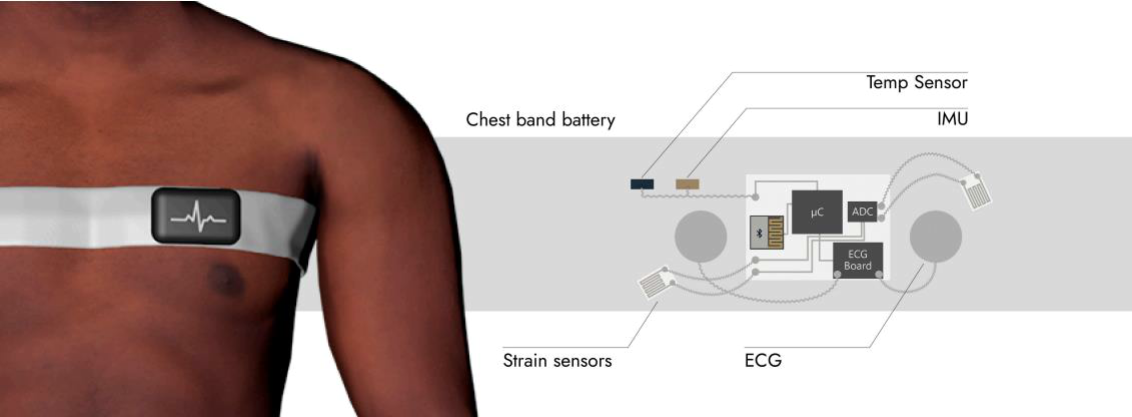
\includegraphics[width=\linewidth]{images/biosticker imgs/test.png}
    \end{minipage}
    \begin{minipage}[l]{0.25\linewidth}
        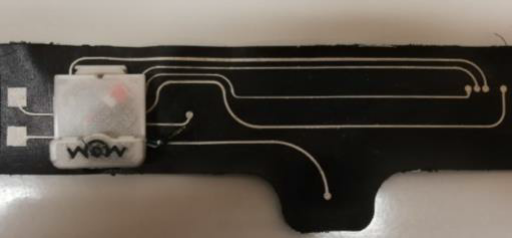
\includegraphics[width=\linewidth]{images/biosticker imgs/a.png}
        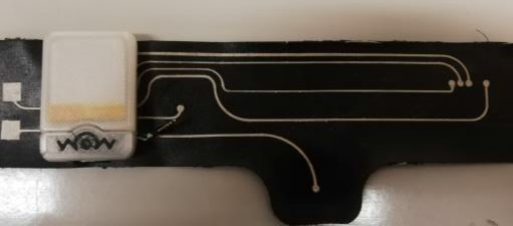
\includegraphics[width=\linewidth]{images/biosticker imgs/b.png}
        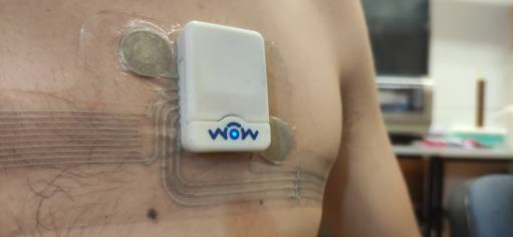
\includegraphics[width=\linewidth]{images/biosticker imgs/c.png}
    \end{minipage}
    \centering
    \caption[Illustration of the \textit{Biostickers}.]{Illustration of the \textit{Biostickers}. On the left, a conceptual illustration of the different components that form the \textit{Biosticker} is shown. On the right, photographies of a test volunteer using the \textit{Biosticker} are exhibited.}
    \label{fig:biosticker-imgs}
\end{figure}


\paragraph{} Additionally, for debugging purposes, researchers at the \acs{ISR} developed a simple developer \acs{UI} to be deployed on the \textit{Smart box}, which can be seen on Figure \ref{fig:smartbox-gui}.

\begin{figure}[H]
    \centering
    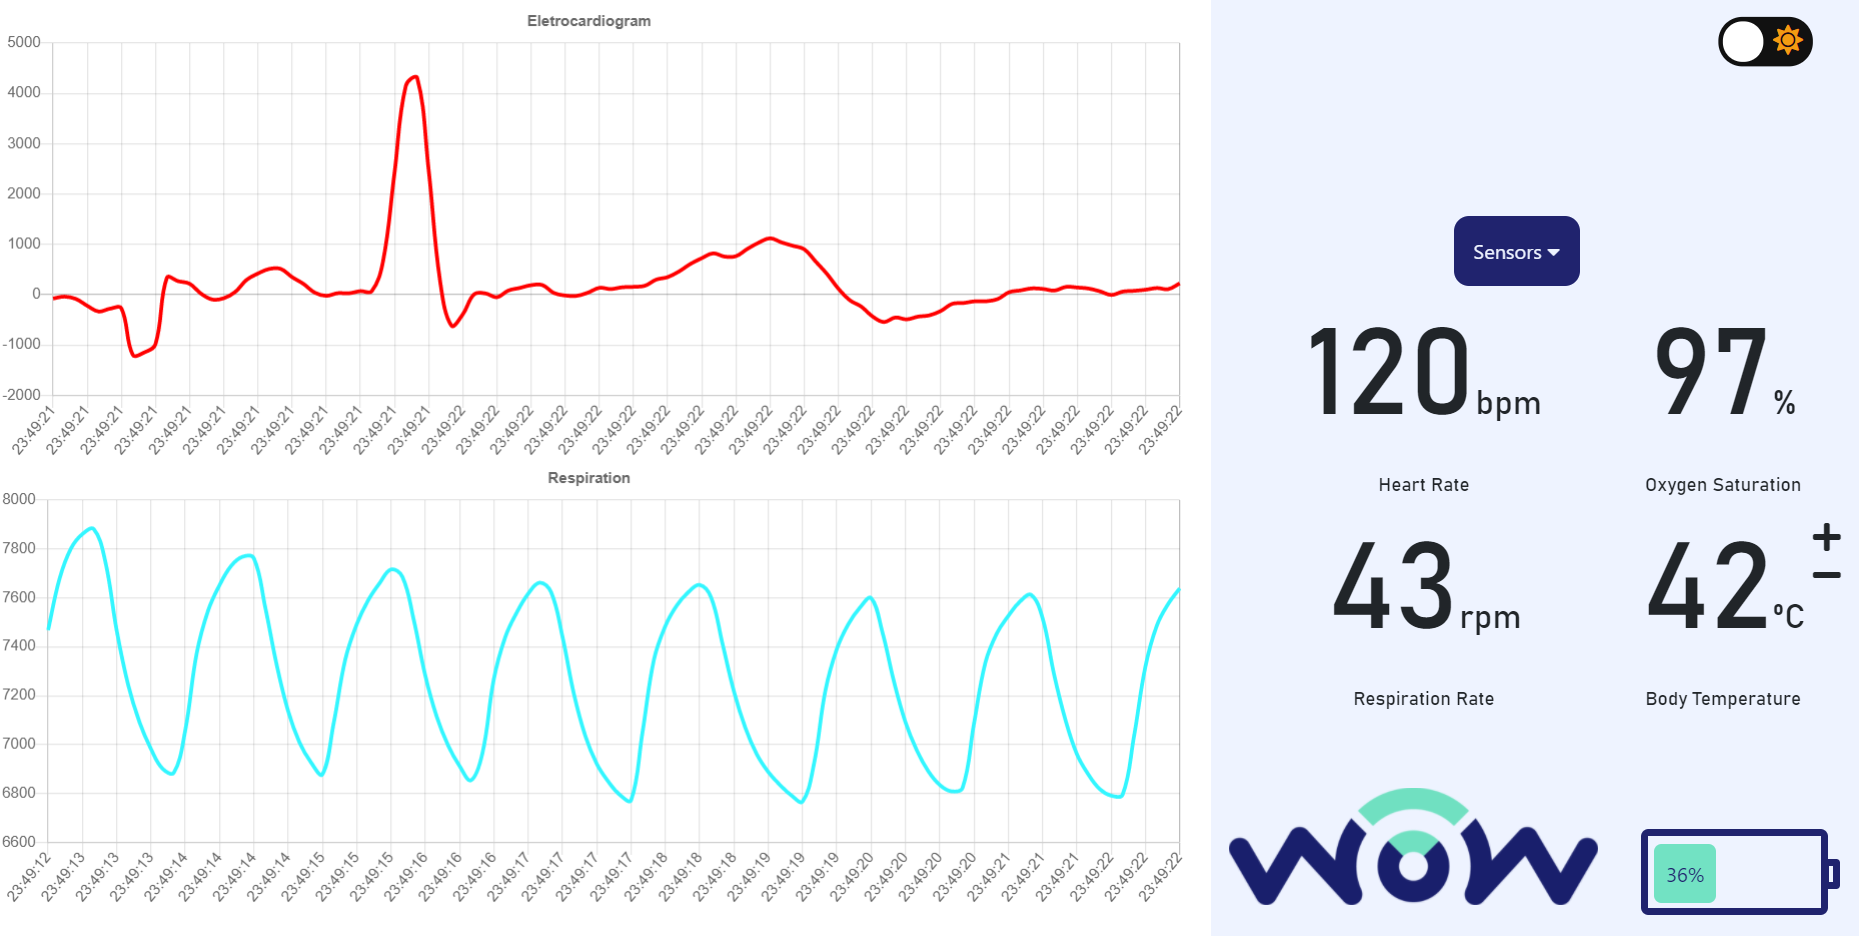
\includegraphics[width=\linewidth]{images/smartbox-gui.png}
    \caption{Illustration of the developer \acs{UI} for debugging the \textit{Smart box} acquisition, designed by the \acs{WoW} research team at \acs{ISR}.}
    \label{fig:smartbox-gui}
\end{figure}

\paragraph{} Regarding data acquisition, the \textit{Smart box} collects 5 distinct biosignals, which can be seen on the developer low level \acs{UI} on Figure \ref{fig:smartbox-gui}:

\label{sec:biosticker_data}

\begin{itemize}
    \item \acf{ECG} -- Byte array (20 byte length) with the electrical signal measured, with a frequency of 20 Hz.
    \item Respiration Rate -- An unsigned integer (4 bytes) representation of the rate of respiration, with a frequency of 10 Hz.
    \item Heart Rate -- An unsigned byte representation of the heart rate in \textit{beats per minute}, every 5s.
    \item Body Temperature -- An IEEE 11073\footnote{\url{https://standards.ieee.org/standard/11073-10207-2017.html}} floating-point number representation of the body temperature, every 60s.
    \item Oxygen Saturation -- A standard floating-point number (4 bytes) representation of the oxygen saturation, every 1s.
\end{itemize}

\section{Deciding on a Hardware Platform}

In the context of this dissertation, two different \acl{SBC}s (\acs{SBC}) have been considered for the development of the \textit{Smart box}: a Raspberry Pi 4 Model B and an UDOO BOLT v3. In the following sections the characteristics of each platform are discussed and compared. 

\subsubsection{Raspberry Pi 4 Model B}

Raspberry Pi denotes a series of \acs{SBC}s which are developed by the Raspberry Pi Foundation, a UK-based charity that aims to educate the general public about the power of computing and digital making, in association with Broadcom. It is one of the most popular hardware platforms used by developers due to its accessible price and community support \cite{jain2021introduction}.
At the time of the writing, the Raspberry Pi 4 Model B (or Raspberry Pi 4B)\footnote{\url{https://www.raspberrypi.com/products/raspberry-pi-4-model-b/}}, which can be seen in Figure \ref{fig:raspberrypi-image}, is the latest revision of the Raspberry Pi series, powered by Broadcom BCM2711 System on a Chip (SoC).

\begin{figure}[H]
    \centering
    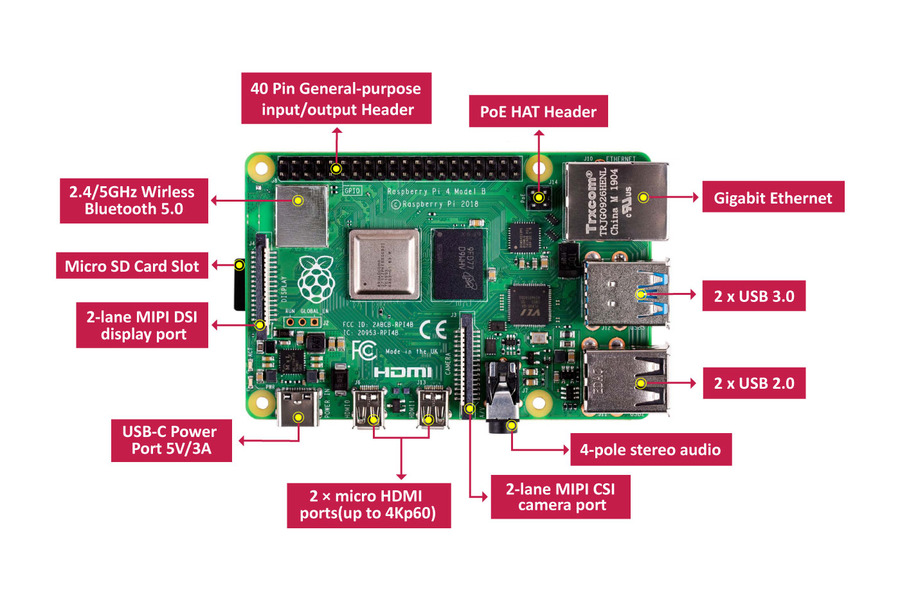
\includegraphics[width=\linewidth]{images/raspberry-4-modele-b-4go.jpg}
    \caption{Raspberry Pi 4B.}
    \label{fig:raspberrypi-image}
\end{figure}

\subsubsection{UDOO BOLT V3}

As stated by the manufacturer\footnote{\url{https://www.udoo.org/discover-the-udoo-bolt/}}, the ``UDOO BOLT is a quantum leap compared to current maker boards''. It represents a series of high performance \acs{SBC}, equipped with the latest generation of AMD Ryzen Embedded SoC. Additionally, it contains an Arduino Compatible microcontroller (connected via UART), making the UDOO BOLT extremely versatile.
UDOO BOLT is incredibly well-supported by UDOO but unfortunately, it still does not have nearly the same community support of Raspberry Pi.

\paragraph{} The UDOO BOLT V3, which can be seen in Figure \ref{fig:udoobolt-image}, is the entry-level product of the series, but it is still capable of allegedly outperforming full-fledged computers such as the Apple MacBook Pro 13", which just goes to show how powerful these \acs{SBC}s can be.

\begin{figure}[H]
    \centering
    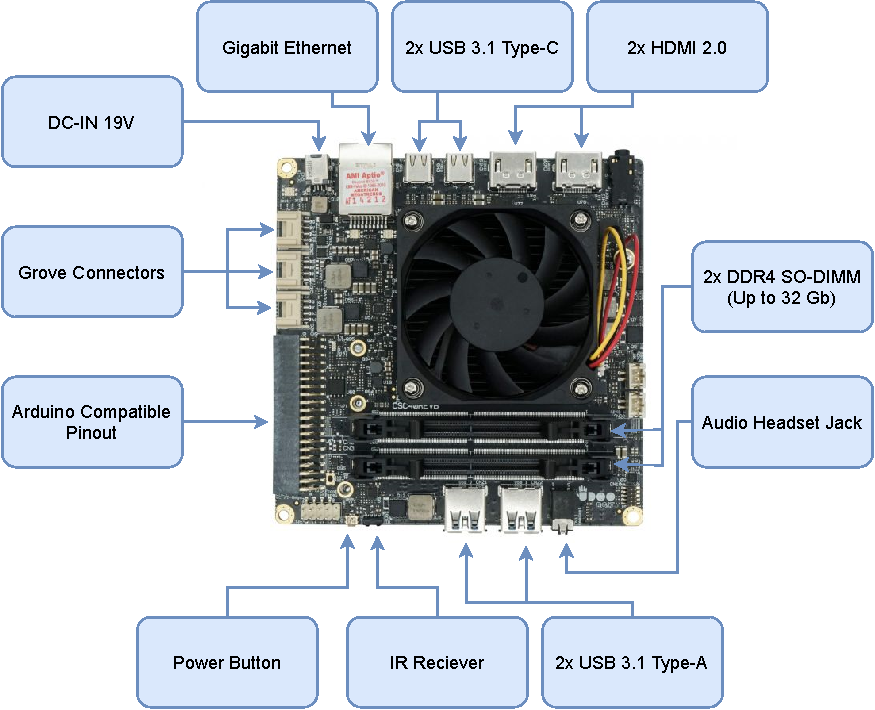
\includegraphics[width=\linewidth]{images/udoobolt-diag.pdf}
    \caption{UDOO BOLT V3.}
    \label{fig:udoobolt-image}
\end{figure}
\clearpage 

\subsection{Comparing the Hardware Platforms}

In order to decide on which platform to pick for the development of the project, it is crucial to compare the specification of both boards, which can be seen in the Table \ref{tab:comparsion-hardwareplatform}.

\paragraph{} From Table \ref{tab:comparsion-hardwareplatform}, it can be concluded that the Raspberry Pi is a much more affordable alternative. At over 1/7 of the price, it already has a working Wi-Fi+BT networking module (which is not included in the UDOO BOLT V3), nearly identical Input/Output (I/O) port capability and a smaller size. UDOO BOLT V3 on the other hand, has a much better SoC, which is expected to deliver a much better overall computing performance.

\renewcommand{\arraystretch}{2.5}
\begin{table}[H]
    \centering
    \caption{Specifications of the Raspberry Pi 4B and UDOO BOLT V3.}
    \begin{adjustbox}{width=0.85\columnwidth,center}
    \begin{tabular}{r|l|l}
        %\textbf{Features} 
        & \textbf{Raspberry Pi 4B}& \textbf{UDOO BOLT V3}  \\ \hline
        \textbf{SoC} &  \makecell{Broadcom BCM2711 \\ (ARMv8 64-bit) \\ 4-core @ 1.5G Hz} & \makecell{AMD Ryzen™ Embedded V1202B \\ (AMD64 64-bit) 2-core @ 2.3G Hz \\ (up to 3.2G Hz turbo)}\\
        \textbf{\acs{RAM}} & 2, 4 or 8 GB LPDDR4 & Up to 32 GB DDR4 (Not included) \\ 
        \textbf{Storage} & \makecell{No internal storage, \\ SDXC Card Support} & \makecell{32 GB internal eMMC + \\1 × SATA III and \\ 2 × M.2 connectors}\\
        \textbf{Networking} & \makecell{2.4/5.0 GHz Wi-Fi, Gigabit \\ Ethernet, Bluetooth 5.0, BLE} & \makecell{Gigabit Ethernet + M.2 Key E slot \\ for optional Wi-Fi+BT module}\\ 
        \textbf{I/O Ports} & \makecell{ 2 × USB 3.0, 2 × USB 2.0, \\ 2 × (Mini) HDMI} & \makecell{2 × USB 3.0 Type-A, \\ 2 × USB Type-C (w/ Display Port \\ + Power Delivery), 2 × HDMI} \\
        \makecell[r]{\textbf{Other} \\\textbf{Features}} & \makecell{Power over Ethernet \\(PoE)–enabled} & \makecell{Includes ATmega32U4 microcontroller\\ (Arduino Leonardo compatible), \\ RTC Battery} \\   
        \textbf{Dimensions} & 8.5 x 5.6 x 1.7 cm & 12 x 12 x 7 cm \\
        \textbf{Price} & \makecell{75.93 € (\textbf{8 GB Model}, \\ including a 32 GB SDXC Card\\ and case)} & \makecell{534.48 € (including external power \\ supply and a 16 GB \acs{RAM} module)} \\
    \end{tabular}
    \end{adjustbox}
    \label{tab:comparsion-hardwareplatform}
\end{table}
\renewcommand{\arraystretch}{1}

\paragraph{} In order to understand how these differences in the hardware specification between the \acs{SBC}s translate to real-world performance, a test suite has been developed and conducted to quantify the performance of each \acs{SBC}. The tools developed for each test can be found here\footnote{\url{https://github.com/WoW-Institute-of-Systems-and-Robotics/smartbox\_benchmark\_tests}}. In the next sections, the details of each test are explained and the performance of each \acs{SBC} is discussed. 

\subsubsection{Test 1: Python Benchmark}

Given the data processing requirements for the \textit{Smart box}, and as Python is used as the main scripting language for most of the \textit{Smart box} development, a simple test has been developed to estimate computing performance, or more specifically (single-threaded) performance of arithmetic tasks, on each \acs{SBC}. In this test, each \acs{SBC} calculates the \textit{n}-th number in the Fibonacci sequence \cite{pierce1951fibonacci}, and the time taken to complete is measured. This process is repeated 10 times for different numbers, from 10000 to 500000, to determine average run time.

\begin{figure}[H]
    \centering
    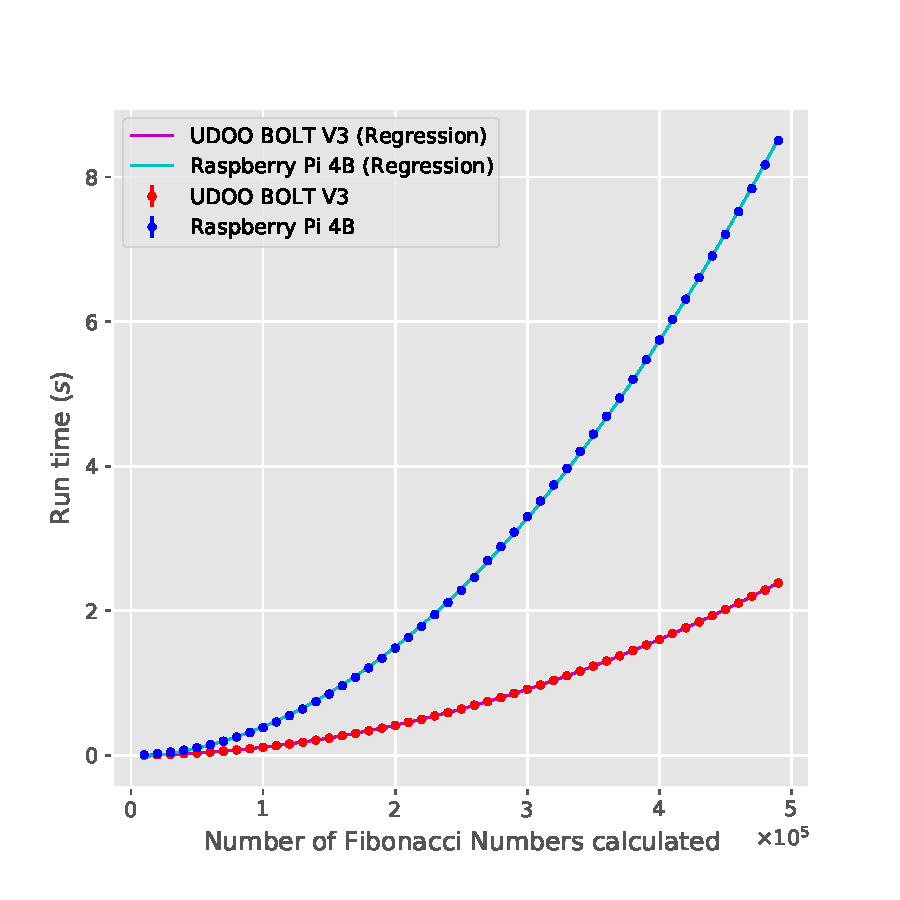
\includegraphics[width=0.67 \linewidth]{images/fibonacci-test.pdf}
    \caption [Custom Python benchmark for the Raspberry Pi 4B and UDOO BOLT V3.]{ Custom Python benchmark for the Raspberry Pi 4B and UDOO BOLT V3.}%The standard deviation for each run time is inferior to point size in each test, and therefore cannot be not displayed in the figure.}
    \label{fig:fibonacci-tests}
\end{figure}

From Figure \ref{fig:fibonacci-tests}, it can be observed that the time taken for computing each number increases quadratically for each platform ($R^2>0.99$ for both regressions), as expected, with UDOO BOLT V3 outperforming Raspberry Pi 4B on average by a factor of 2.5 $\pm$ 0.2.


% However, this phenomenon is unexpected due to the nature of the algorithm implemented, which is an iterative Fibonacci algorithm with a linear time complexity ($O(n)$). One factor which could influence the computation time is the overheating of hardware components, as these synthetic benchmarks produce a considerable \acs{CPU} load and take some time to execute (almost 30 minutes on Raspberry Pi 4B). These tests were conducted with the \acs{SBC}s already ``warmed'' by executing running this test multiple times prior to recording the data, but it  


\subsubsection{Test 2: Phoronix Test Suite}

The Phoronix Test Suite\footnote{\url{https://www.phoronix-test-suite.com/}} is an open-source benchmarking platform used for comparing the performance of different systems. The framework provides compilations of tests for a variety of tools and is also fully customizable and expandable, allowing users to develop and automate their own tests in a clean, reproducible and easy-to-use fashion. The test profiles work by measuring some property of the benchmark, (\textit{e.g.} the run time for calculating the first 100 Fibonacci numbers) and use it to provide an estimate of the performance of the \acs{SBC}, which can be easily used for comparison between different systems. 

\paragraph{} For the purposes of evaluating the computing performance of each \acs{SBC}, the following standard test profiles provided by Phoronix\footnote{\url{https://openbenchmarking.org/}} were chosen, which are a compilation of the most popular Python and \acf{CPU} benchmarks used\footnote{The benchmark results obtained were published in the \textit{OpenBenchmarking.org} website, and can be found in the following URL: \url{https://openbenchmarking.org/result/2110255-JNCF-211025851}.}:

\begin{itemize}
    \item BYTE Unix Benchmark (``BYTE''), single-threaded \acs{CPU} benchmark -- Runs BYTE UNIX benchmark suite (more accurately, the Dhrystone 2 synthetic benchmark) to measure the amount of instructions per second (IPS). 
    \item 7-Zip Compression (``7-Zip''), multithreaded \acs{CPU} benchmark -- Runs the benchmark feature integrated in 7-Zip to measure the amount of millions instructions per second (MIPS). The benchmark consists of a LZMA data compression and decompression test run, using all available threads in the system (meaning it will scale highly with the amount of threads in the system). 
    \item PyBench Benchmark (``PyBench''), single-threaded Python \& \acs{CPU} benchmark -- Executes different function such as built-in function calls and nested for-loops and measures its runtime.
    \item PyPerformance \textit{chaos} Benchmark (``chaos''), single-threaded Python \& \acs{CPU} benchmark -- Create chaos game-like fractals \cite{Jeffrey1992} and measures its run-time. 
    \item PyPerformance \textit{float} Benchmark (``float''), single-threaded Python \& \acs{CPU} benchmark -- Create 100,000 random floating-point numbers and calculate the co-sine, sine and square root of each one and measures its run-time.
    \item PyPerformance \textit{nbody} Benchmark (``nbody''), single-threaded Python \& \acs{CPU} benchmark -- Runs an \textit{n-body} problem simulation \cite{Playne2009} and measures its run-time.
    \item PyPerformance \textit{json\_loads} Benchmark (``json''), single-threaded Python \& \acs{CPU} benchmark -- Evaluates \acf{JSON}\footnote{The JavaScript Object Notation (JSON) Data Interchange Format: \url{https://www.rfc-editor.org/rfc/rfc8259.html}} parsing and serialization, a widely used open standard data format, by dumping and loading thousands of objects and measures its runtime.
    \item PyPerformance \textit{crypto\_pyaes} Benchmark (``crypto''), single-threaded Python \& \acs{CPU} benchmark -- Runs the AES block-cipher Python implementation and measures its run-time.
    \item PyPerformance \textit{regex\_compile} Benchmark (``regex''), single-threaded Python \& \acs{CPU} benchmark -- Compiles different \textit{regular expressions} or \textit{regexes} in Python and measures its run-time.
    \item PyPerformance \textit{python\_startup} Benchmark (``startup''), single-threaded Python \& general system performance benchmark -- Measures Python's startup time.
    \item PyPerformance \textit{django\_template} Benchmark (``django''), single-threaded Python benchmark -- Builds a 150x150-cell HTML table and measures its run-time.
\end{itemize}

\clearpage 

\begin{figure}[H]
    \centering
    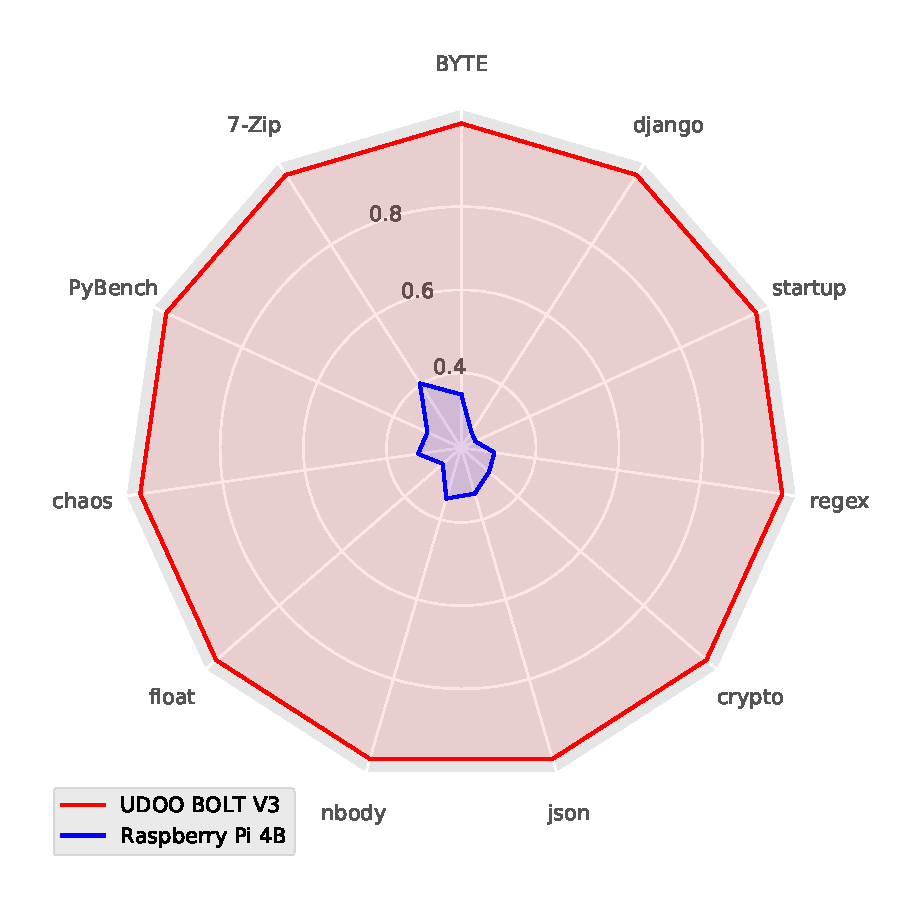
\includegraphics[width=0.6 \linewidth]{images/phoronix-benchmarks.pdf}
    \caption [Phoronix benchmarks for the UDOO BOLT V3 and Raspberry Pi 4B.]{ Phoronix benchmarks for the UDOO BOLT V3 and Raspberry Pi 4B. The performance values for each test are normalized to UDOO BOLT V3 performance.}
    \label{fig:phronix-benchmarks}
\end{figure}

%\todo[inline]{To-do: Review this analysis later.}
% ok discutiste o 7-Zip, e os outros?
% Por ex: o BYTE tb n está longe de 0.4 e é single threaded. E a disparidade (resultados mt piores) no startup e float? consegues discutir (mesmo que especulando) o porquê de isto acontecer?

\paragraph{} From Figure \ref{fig:phronix-benchmarks}, it can be observed that UDOO BOLT V3 performs much better than Raspberry Pi 4B in every benchmark, as expected. However, some disparity in the relative performance throughout the benchmarks is also noticed. 

\paragraph{} For example, in the 7-Zip benchmark, this is likely due to the fact that is a multithreaded test, and as Raspberry Pi 4B has more threads than UDOO BOLT V3, it manages to close the performance gap (albeit only slightly). For the \textit{startup} and \textit{django} benchmark score differences, these are mostly affected by the load time of the Python interpreter, which is significantly affected by the main storage device. A high-speed SD card was used with the Raspberry Pi and the internal eMMC storage was used with the UDOO BOLT V3, which is a significantly faster storage medium than an SD card and thus is most likely the cause for the benchmark score difference. Benchmarks which use many arithmetic operations, like the \textit{float} benchmark or \textit{BYTE}, can also show significantly different results as well since each \acs{CPU} architecture has different optimizations for handling floating point operations or integers operations.

\paragraph{} On average, UDOO BOLT V3 outperforms Raspberry Pi 4B in all benchmarks by a factor of 2.21 $\pm$ 0.4.

\subsubsection{Test 3: \acs{MQTT} Benchmark}

As the \textit{Smart box} is intended to communicate with the \textit{Smart Gateway} through \acs{MQTT} messages, an evaluation of how each system handles the load associated with a \acs{MQTT} client is performed. For this test, each \acs{SBC} uses a simple \acs{MQTT} client, that subscribes to a single topic and publishes a message that same topic for different transmission rates, with a payload with a length of 1000 bytes, through a \acs{MQTT} broker in the local network. Additionally, the tests measure the communication with and without \acs{TLS} to evaluate the impact of the secure protocol.

\begin{figure}[H]
    \centering
    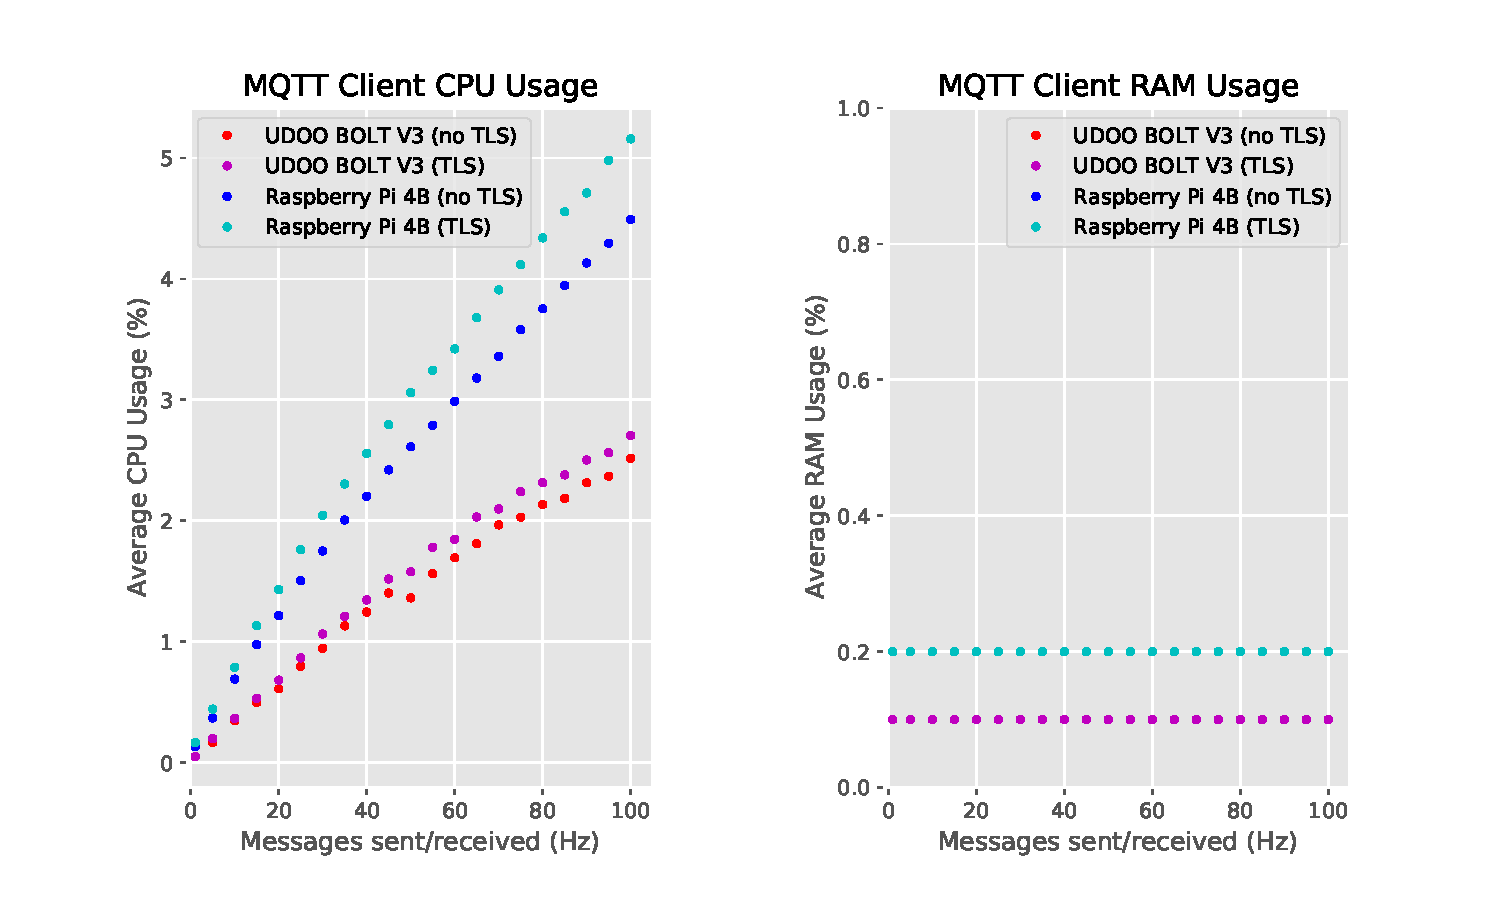
\includegraphics[width=\linewidth]{images/mqtt_test_results.pdf}
    \caption[\acs{MQTT} benchmark for Raspberry Pi 4B and UDOO BOLT V3.]{\acs{MQTT} benchmark for Raspberry Pi 4B and UDOO BOLT V3. In the \acs{RAM} usage graph, the tests with TLS and no TLS show identical results, causing the data points to overlap.}
    \label{fig:mqtt-tests}
\end{figure}

\paragraph{} The \acs{MQTT} client is a very lightweight process, and as seen in Figure \ref{fig:mqtt-tests}, it is capable of running on both platforms with trivial performance impact. As the transmission frequency increases, the \acs{CPU} load increases linearly, Additionally, it can be observed that the Raspberry Pi uses more \acs{CPU} than the UDOO BOLT V3, by a factor of $1.88 \pm 0.21$ without using \acs{TLS} and $2.01 \pm 0.31$ using \acs{TLS}. The usage of \acs{RAM} remains constant throughout the tests, 0.1\% on UDOO BOLT V3 and 0.2\% on Raspberry Pi 4B -- which are very negligible values, and thus do not represent any significant impact in performance. Additionally, the usage of \acs{TLS} directly impacts the performance of the devices, but not to any significant degree -- $0.16\% \pm 0.02$ more \acs{CPU} usage on the Raspberry Pi and $0.094\% \pm 0.039$ on UDOO BOLT V3.

\paragraph{} Overall, the UDOO BOLT V3 shows a much better results, with nearly twice less \acs{CPU} and \acs{RAM} usage. However, even at transmission and reception rate of 100 Hz, the resource usage of both devices is very minimal (<6\%) and thus should not meaningfully impact real-world performance.

\subsection{Final Decision on Smart box hardware}

Based on the results of our tests it is concluded that the UDOO BOLT V3 heavily outperforms the Raspberry Pi 4B in \acs{CPU} benchmarks, but shows a negligible difference in memory usage. Nonetheless, these performance gains do not meaningfully impact the \textit{Smart box} functionality, for example, in the \acs{MQTT} communication. This observation can also be extended to other functionalities, such as the developer \acs{UI} or the Python acquisition script, which should have a similar resource load to the \acs{MQTT} client in the \acs{MQTT} benchmark, so both \acs{SBC}s are more than capable of assuring the necessary functions.

\paragraph{} Additionally, the Raspberry Pi 4B comes out of the box with an included Wi-Fi+\acs{BLE} combo networking card, 8 GB of \acs{RAM} (as the 8 GB model was chosen), and a much smaller form factor -- which is very useful for embedding the \textit{Smart box} in the \textit{SmartBeds}. And this is at 1/7 the cost of UDOO BOLT V3, making this much more affordable to scale and replicate the system with many \textit{Smart boxes}.

\paragraph{} Due to all the aforementioned reasons, Raspberry Pi 4B was chosen for the \textit{Smart box} development in the scope of the \acs{WoW} project.

\section{Communication with the Biostickers}

As previously mentioned, the communication between the \textit{Biostickers} and the \textit{Smart box} makes use of the \acs{BLE} protocol. One of the advantages of using the Raspberry Pi 4B, as discussed in the previous section, is the fact that it already includes all networking functionality needed for the project. 

\paragraph{} However, the communication with the \textit{Biostickers} is very critical and demanding. During the development of the project, the research team has decided to use a \textit{Biosticker} coupled with a commercially available Pulse Oximeter%\footnote{\url{https://www.proactmedical.co.uk/product/creative-pc-60fw-finger-pulse-oximeter-with-bluetooth}} 
-- used to measure oxygen saturation at the fingertip --  in order to capture all required biosignals. This means that the \acs{BLE} acquisition system must be capable of handling both communications simultaneously. With this in mind, it is necessary to verify if the included \acs{BLE} adapter of the Raspberry Pi board is sufficient for the task, or if a different acquisition hardware should be considered instead.

\paragraph{} In order to understand how data transmission works between \acs{BLE} devices, some technical background regarding the data transmission in protocol is presented.

\subsection{Technical Background} 
The \acs{BLE} protocol stack is organized into three major components, as shown in Figure \ref{fig:ble-protocol-stack}: the Application Layer, the Host Layer and Controller Layer. 

\begin{figure}[H]
    \centering
    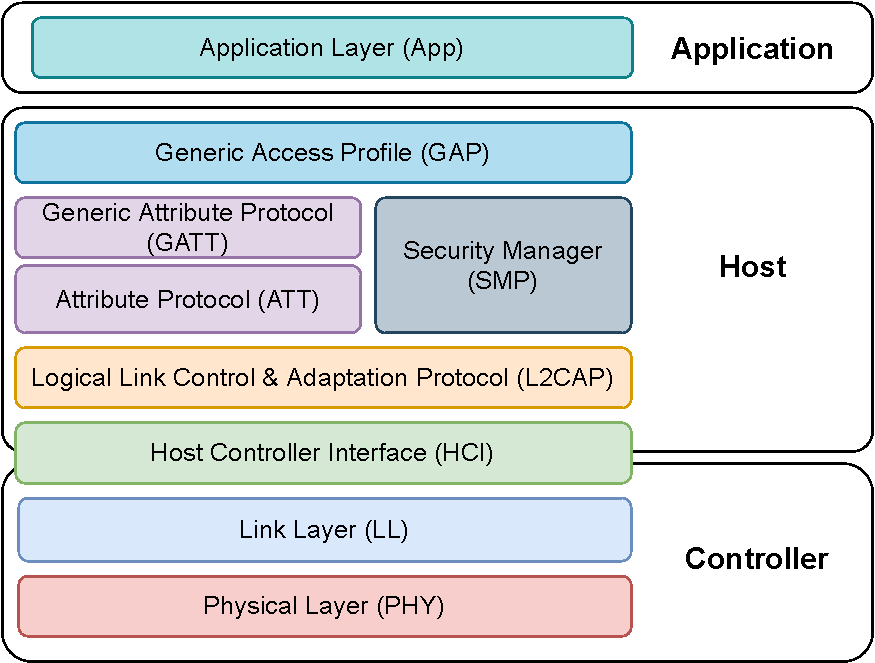
\includegraphics[width=0.6\linewidth]{images/ble protocol stack.pdf}
    \caption[Diagram of the different components of the \acs{BLE} protocol stack.]{Diagram of the different components of the \acs{BLE} protocol stack. Adapted from \cite{Specification1999, Farej2020}}
    \label{fig:ble-protocol-stack}
\end{figure}

The \acf{PHY} and \acf{LL} components constitute the Controller layer. The \acs{PHY} is the bottom layer of the \acs{BLE} stack, and is responsible for the transmission and reception of information over radio waves on the Industrial Scientific Medical 2.4GHz band. According to the latest revision of the specification \cite{Specification1999}, \acs{BLE} supports 3 distinct physical layers: LE 1M, LE 2M and LE Coded. Each of these define which modulation speed (1 Msym/s or 2 Msym/s) and which coding scheme (S=1,2 or 8 bits) is used. LE 1M is the default \acs{PHY} which must be supported by \acs{BLE} devices, with a bit rate of 1 Mbps (1Msym/s with S=1). In the latest major revision of Bluetooth, the latter two \acs{PHY}s were introduced: LE 2M doubles the bit rate to 2 Mbps using a faster modulation scheme (2 Msym/s with S=1), whereas LE Coded has a much larger range (2x or 4x compared to LE 1M), at cost of a lower bit rate (500 kbps or 125 kbps) by using a different coding scheme (1 Msym/s with S=2 or 8 bits respectively). 

The \acf{LL} interfaces directly with the \acs{PHY}, and manages the link state of the radio. It also provides the mechanism for the higher layers to interact with the radio transceiver. 

\paragraph{} Following the \acf{LL} is the Host Layer, containing the higher level components of the protocol stack that interact with the application level layers. The \acs{L2CAP} is responsible for managing the data between the \acs{LL} through the \acf{HCI} and the higher layers in the protocol stack. It abstracts the communication details from the higher layers, handling seamlessly the fragmentation of the data into multiple \acs{LL} data packets for transmission and reassembly of \acs{LL} data packets for higher layer protocols, such as the \acf{ATT}.

\acs{ATT} is the protocol used to expose the application data to other \acs{BLE} devices through data structures called ``attributes'', which are the smallest addressable units of data used by \acs{ATT}. These entail three main properties \cite{Specification1999}: 

\begin{itemize}
    \item An attribute type, defined by a \acf{UUID}\footnote{\url{https://tools.ietf.org/html/rfc4122}}, which indicates the type of data that is stored in the attribute.
    \item An attribute handle, to uniquely identify that attribute on the device (which in this case assumes the role of a server), allowing other devices (which assume the role of clients) to refer the attribute for read and write requests;
    \item A set of permissions which limit the types of interactions.
\end{itemize}

\paragraph{} However, from the application point of view, data is exchanged using \acf{GATT}. \acs{GATT} defines a service framework using the \acs{ATT} protocol, with the procedures used to exchange data between the \acs{BLE} devices. Regarding \acs{GATT}, there are three main constructs to consider:

\begin{itemize}
    \item \acs{GATT} Characteristic -- The lowest level concept in \acs{GATT} transactions is the Characteristic, which encapsulates a single data point, \textit{e.g.} a temperature measurement, an accelerometer reading, etc. It also defines the different types of interactions, such as reading, writing, subscribing for notifications, etc.
    \item \acs{GATT} Service -- A collection of \acs{GATT} characteristics.
    \item \acs{GATT} Profile -- A collection of Services, usually predefined by Bluetooth \acf{SIG} in order to promote interoperability, which may also be customized for the application's needs.
\end{itemize}

\paragraph{} The \acf{SMP} handles security in data transmissions, containing the security algorithms used to encrypt and decrypt the communication. %For \acs{BLE} connections, there are 2 security modes (and in each mode levels that determine the degree of security) which supports different security functionalities, such as pairing, encryption and data integrity at different layers of the \acs{BLE} stack. Table \ref{tab:ble-security-modes} lists the support for security features in each security mode.

%\begin{table}[H]
    %\centering
    %\caption[Overview of security features in \acs{BLE}.]{ Overview of security features in \acs{BLE}. Source \cite{Gomez2012}.}
    %\begin{adjustbox}{width=\columnwidth,center}
    %\begin{tabular}{l|l|l|l|l|l}
    %        &                  & \textbf{Pairing} & \textbf{Encryption} & \textbf{Data Integrity} & \textbf{Layer}              \\ \hline
    %\multirow{3}{*}{\textbf{LE Security Mode 1}} & \textbf{Level 1} & \xmark           & \xmark              & \xmark                  & \multirow{3}{*}{Link Layer} \\
   %         & \textbf{Level 2} & Unauthenticated  & \cmark              & \cmark                  &                             \\
  %          & \textbf{Level 3} & Authenticated    & \cmark              & \cmark                  &                             \\ \hline
  %  \multirow{2}{*}{\textbf{LE Security Mode 2}} & \textbf{Level 1} & Unauthenticated  & \xmark              & \cmark                  & \multirow{2}{*}{ATT Layer}  \\
  %          & \textbf{Level 2} & Authenticated    & \xmark              & \cmark                  &                            
 %   \end{tabular}
%    \end{adjustbox}
%    \label{tab:ble-security-modes}
%\end{table}

\paragraph{} Finally, the Application Layer contains the user application, which interfaces with the Bluetooth protocol stack.

% \paragraph{} After this overview of the different layers that compose the \acs{BLE} stack, we are ready to engage in the analysis of the \acs{BLE} data transmission.

\subsubsection{\acs{BLE} data transmission}

\paragraph{} Before discussing \acs{BLE} data transmissions, it is important to introduce to certain terminology which is commonly used:

\begin{itemize}
    \item Central device (or master): Device that initiates commands and requests.
    \item Peripheral device (or slave): Device that receives commands and requests, and returns responses.
    \item Connection Event: Moment of the connection where the devices engage in radio transmissions.
\end{itemize}

\paragraph{} As seen previously, there are multiple layers that are involved in the transmission of data in \acs{BLE}. Figure \ref{fig:ble-ll-packet-format} displays the format of a \acs{BLE} data packet, showing how the data is encapsulated for the transmission.

\begin{figure}[H]
    \centering
    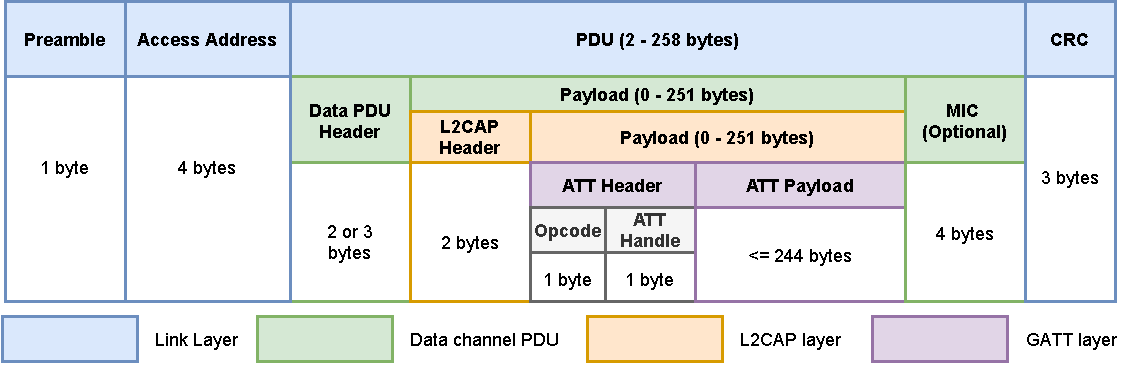
\includegraphics[width=\linewidth]{images/bluetooth data packet format.pdf}
    \caption[Diagram of the \acs{BLE} data packet format for LE 1M \acs{PHY}.]{\acs{BLE} data packet format for an \acs{ATT} write message using LE 1M \acs{PHY}. Adapted from \cite{Specification1999, Farej2020}. The Message Integrity Check (MIC) and Cyclic Redundancy Check (CRC), which are not discussed above, are used for validating the integrity of the data packet.}
    \label{fig:ble-ll-packet-format}
\end{figure}

\paragraph{} Communication in \acs{BLE} works in a particular manner. Instead of having the devices transmit data whenever there is new information to exchange, the devices group their radio transmissions in a brief time frame that occurs periodically, called the Connection Event \cite{Specification1999}. This allows devices to heavily reduce power consumption, as they can negotiate the amount of radio ``downtime'' to minimize the amount of transmissions.

\paragraph{}  Figure \ref{fig:ble-message-sequence-chart} illustrates a Connection Event during a \acs{BLE} communication between two devices exchanging a single message, A and B. When the device A wants to communicate to the device B, the data must be first fragmented into different \acs{LL} data packets on the \acs{L2CAP} layer, which for this simple example is not considered. The data is transmitted to device B through the \acs{LL} layer, and the data is then reassembled on device B. When the packet is received on device B, it must send a transmission to device A acknowledging the reception of the packet (which contains an empty payload), as device A can only continue transmitting after receiving the acknowledgement \cite{Specification1999}.


\begin{figure}[H]
    \centering
    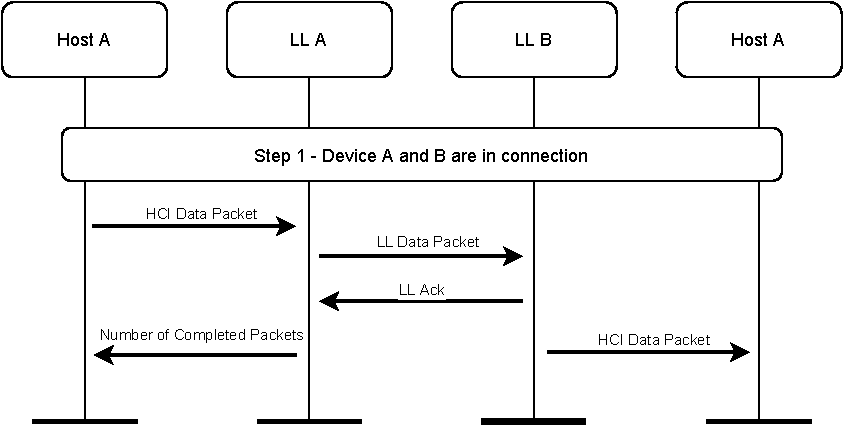
\includegraphics[width=\linewidth]{images/ble-sending-data.pdf}
    \caption[Message sequence chart between two \acs{BLE} devices during a Connection Event.]{Message sequence chart between two \acs{BLE} devices during a Connection Event. Adapted from \cite{Specification1999}.}
    \label{fig:ble-message-sequence-chart}
\end{figure}

\paragraph{} Multiple parameters guide how \acs{BLE} data connections are performed \cite{Specification1999}, which are the following: 
\begin{itemize}
    \item Slave Latency: Number of consecutive connection events that the slave device is not required to listen for the master. It allows a slave to use a reduced number of connection events, thus minimizing power consumption.
    \item Connection Interval: Time between two consecutive connection events.
    \item Supervisor Timeout: Maximum time between two received data \acl{PDU}s (\acs{PDU}) before the connection is considered lost.
    \item \acf{MTU} for the \acs{ATT} protocol: Length of the \acs{PDU} for the \acs{ATT} protocol, which includes the \acs{ATT} header as well as the payload containing the data to be transmitted.
    \item Connection \acs{PHY}: Modulation and coding scheme used for the connection.
\end{itemize}

\subsubsection{\acs{BLE} protocol stack on Linux} 

In the \acs{WoW} project, the data acquisition has been developed using the official Linux implementation of the \acs{BLE} protocol stack \cite{BlueZ} -- \textit{BlueZ} -- in order to promote interoperability; since these drivers are developed and used by the community, allowing us to use multiple \acs{BLE} adapters, and even different \acs{SBC}s, using the same codebase without being tied down to proprietary code. 

% \paragraph{} Currently, \textit{BlueZ} only officially supports up to the Bluetooth 4.2 specification, which is, at the time of writing, is still the predominantly used version \cite{Faria2020}. Nonetheless, Bluetooth specifications are generally backwards compatible with older versions.

% \todo[inline]{Nota para @David Portugal: Isto é o que está indicado no website, mas existem funcionalidades de Bluetooth 5.X que estão implementadas (mas não especificam o escopo que está implementado). Indico alguma coisa sobre isso? Removo este parágrafo? Ou deixo tudo como está? }


\subsection{Choosing a \acs{BLE} adapter} 

\paragraph{} As mentioned previously, one of the objectives of this dissertation work is to analyze if the internal \acs{BLE} adapter provided by the Raspberry Pi 4B is sufficient for the \acs{WoW} project. To achieve this, the adapter is compared with another commercially available adapter that met the requirements for the project. These are the following:

\begin{itemize}
    \item The adapter must support, at least, the Bluetooth 5.0 core specification.
    \item The adapter must natively support Ubuntu 20.04 LTS, as well as the \textit{BlueZ} \acs{BLE} protocol stack. 
    %\item The adapter should support the LE 2M physical layer for better throughput.
\end{itemize}

\paragraph{} After investigating the available market, the ASUS USB-BT500 USB adapter\footnote{\url{https://www.asus.com/Networking-IoT-Servers/Adapters/All-series/USB-BT500/}} was chosen due to its affordability and availability, making it an adequate fit for the project's needs.

\paragraph{} In the next section, multiple tests are conducted to evaluate the performance of ASUS USB-BT500 against the internal \acs{BLE} adapter in the Raspberry Pi 4B to reach a decision on which BLE adapter hardware should be used for the transmission of data from the \textit{Biosticker} to the \textit{Smart box}.

\subsection{Testing \acs{BLE} Communication} 

To ensure that a \acs{BLE} adapter is capable of handling the communication on the \textit{Smart box}, two different tests were designed to evaluate their performance at different distances: 

\renewcommand{\labelenumi}{\textit{\alph{enumi})}}

\begin{enumerate}
    \item A test to evaluate the roundtrip time for a single message (for different sizes).
    \item A test to evaluate the maximum bandwidth achievable at a given distance. 
\end{enumerate}
\renewcommand{\labelenumi}{\arabic{enumi}.}

\paragraph{} For these tests, it should be ensured that the conditions are very similar to those when acquiring data from the \textit{Biostickers}. To this end, the same microcontroller is used -- nRF52832 \acs{SoC} -- which is used in the \textit{Biostickers}, with our own custom firmware for the tests. Therefore, the device which is used for the tests is the nRF52-DK developer kit\footnote{\url{https://www.nordicsemi.com/Products/Development-hardware/nrf52-dk}}. The firmware for the microcontroller is built using the latest version of MbedOS\footnote{\url{https://os.mbed.com/mbed-os/}}, an operative system for ARM-based microcontrollers, and can be found here\footnote{\url{https://github.com/WoW-Institute-of-Systems-and-Robotics/ble-test-firmwares/}}.

\subsubsection{Test Conditions}
\label{sec:ble_test_conditions}
\paragraph{} During the preparation and development of these tests, it was discovered that the ASUS USB-BT500 supported an optional functionality which was not documented in its specification -- \acf{DLE}. This feature, introduced in Bluetooth 4.2, allows \acs{LL} data packet payloads to increase significantly in size, up to 251 bytes (compared to the 23 bytes when not using this feature). It is also worth noting out of the 251 bytes, only 244 bytes can be used after taking into account the \acs{L2CAP} and \acs{ATT} overhead in the data packet for write requests, as seen in Figure \ref{fig:ble-ll-packet-format}.

\paragraph{} Additionally, LE 2M or LE Coded could not be used for the tests as the \acs{BLE} stack seemingly did not support these features, despite claiming support for them and all devices used supporting these features. % In these tests, the security level used was the same as in the \textit{Biostickers}, which is LE Security Mode 1 Level 2.

\paragraph{} In order to ensure replicability and reliability of the test results, the same connection parameters are used for all tests, which are the following:

\begin{table}[H]
    \centering
    \caption{\acs{BLE} connection parameters used for the ASUS USB-BT500 adapter.}
    \begin{tabular}{|l|l|}
    \hline
    \textbf{Connection Interval} & 7.5 ms \\ \hline
    \textbf{Slave Latency}       & 0     \\ \hline
    \textbf{Supervisor Timeout}  & 500 ms \\ \hline
    \textbf{\acs{ATT} \acs{MTU} Length}      & 247 bytes   \\ \hline
    \textbf{\acs{PHY}}      & LE 1M   \\ \hline
    
    \end{tabular}
    \label{tab:ble-connection-values-hci1}
\end{table}

\begin{table}[H]
    \centering
    \caption{\acs{BLE} connection parameters used for internal Raspberry Pi 4B adapter.}
    \begin{tabular}{|l|l|}
    \hline
    \textbf{Connection Interval} & 7.5 ms \\ \hline
    \textbf{Slave Latency}       & 0     \\ \hline
    \textbf{Supervisor Timeout}  & 500 ms \\ \hline
    \textbf{\acs{ATT} \acs{MTU} Length}      & 23 bytes   \\ \hline
    \textbf{\acs{PHY}}      & LE 1M   \\ \hline
    \end{tabular}
    \label{tab:ble-connection-values-hci0}
\end{table}

\paragraph{} These tests were conducted indoors, with the devices (the \acs{BLE} adapter and the microcontroller) in clear view of each other. All tests were performed at different distances: 0, 3, 6 and 9 meters. For distances greater than 9 meters the communication was observed to be too unstable for both adapters. Figure \ref{fig:ble-test-setup} ilustrates the setup used for all \acs{BLE} tests.

\begin{figure}[H]
    \centering
    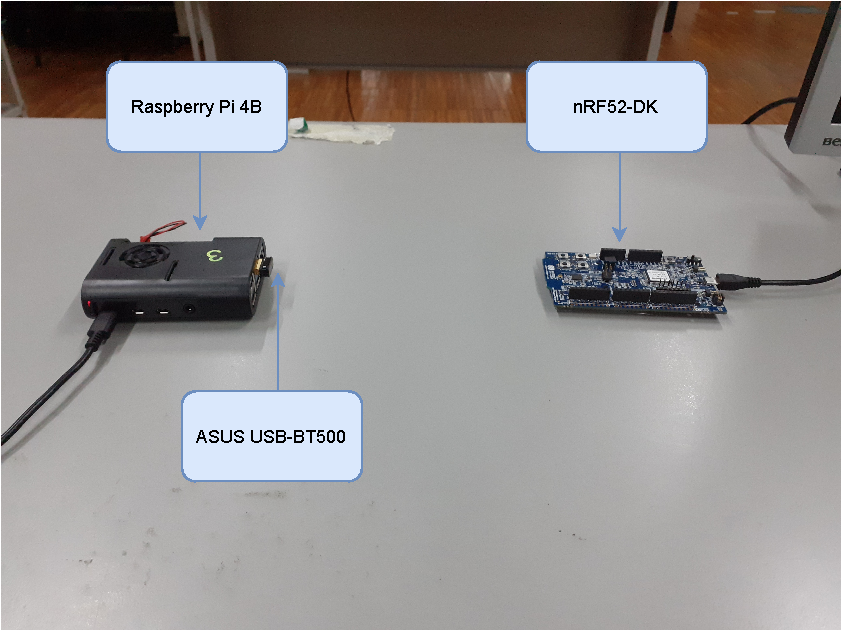
\includegraphics[width=0.75\linewidth]{images/ble test setup.pdf}
    \caption{Setup used for all \acs{BLE} tests.}
    \label{fig:ble-test-setup}
\end{figure}

\subsubsection{Test 1: Roundtrip Time Measurement}

\paragraph{} In this first test, the roundtrip time of a single \acs{ATT} data packet on a \acs{BLE} connection is measured for different payload sizes. For this test, the nRF52-DK board exposes a custom \acs{GATT} service containing 2 characteristics: one is updated by the \textit{Smart box} (characteristic ``A''), and one to which the \textit{Smart box} subscribes for notifications (characteristic ``B''). When the \textit{Smart box} writes on characteristic ``A'' on the nRF52-DK \acs{GATT} server, the \acs{GATT} server changes the value of the characteristic ``B'', which triggers the transmission of a notification to the \textit{Smart box}. Thus, the roundtrip time measured is the time taken between the write request on characteristic ``A'' and the reception of the notification of characteristic ``B''. 

\paragraph{} The roundtrip time is measured for different \acs{ATT} payload lengths, from 1 byte to the maximum size supported by the adapter in 2 byte increments -- \textit{i.e.} payload size $ps=\{1,3,5,\dots\ , 19\}$ bytes for the internal Raspberry Pi 4B and  $ps=\{1,3,5,\dots\ , 243\}$ for ASUS USB-BT500, and for different distances $d={0,3,6,9}$ m. Each test configuration (\textit{i.e.} payload size and distance) has been run 5 times to ensure the consistency of the results, for a total of 2640 independent tests. 
Figures \crefrange{fig:ble-roundtrip-hci1-0m}{fig:ble-roundtrip-hci0-9m} show the average values measured and their standard deviations for different distances. 

\begin{figure}[H]
    \centering
    \begin{minipage}{0.45\linewidth}
        \centering
        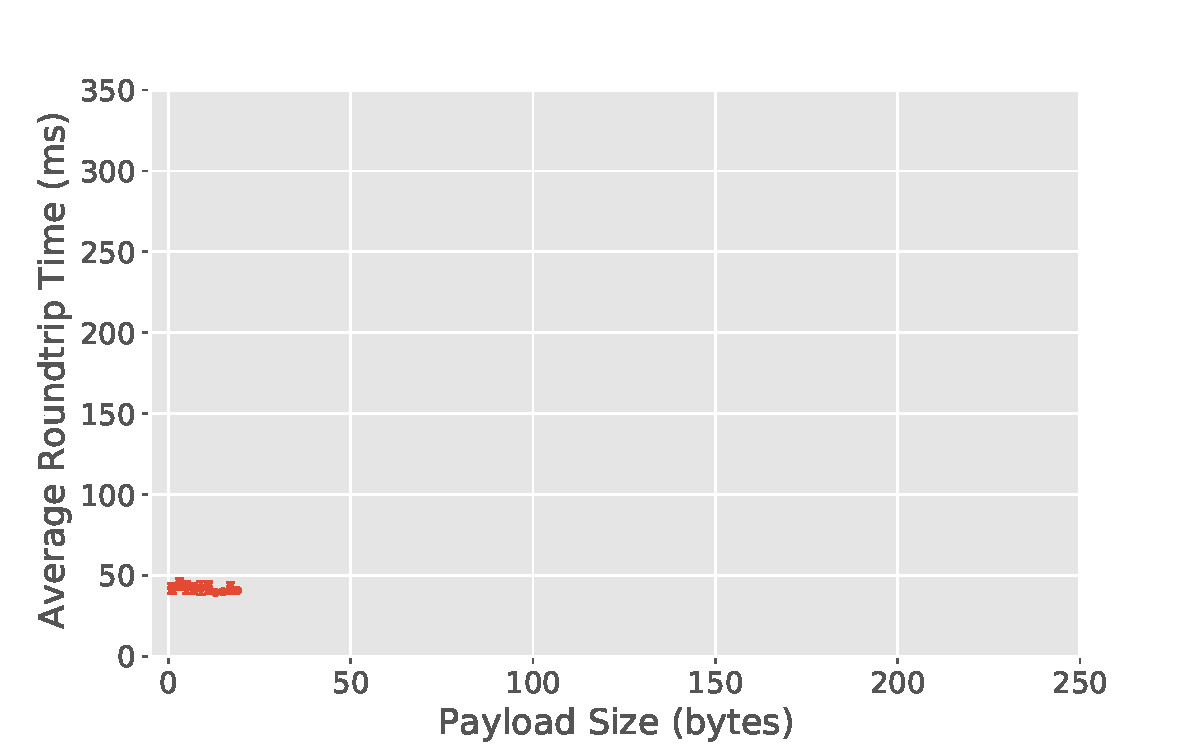
\includegraphics[width=\linewidth]{images/ble-roundtrip-hci1-0cm.pdf}
        \caption[Average \acs{BLE} connection roundtrip time obtained using the Raspberry Pi 4B's internal \acs{BLE} adapter at a distance of 0 m.]{Average \acs{BLE} connection roundtrip time obtained using Raspberry Pi 4B's internal \acs{BLE} adapter at a distance of $0\text{ m}$.}
        \label{fig:ble-roundtrip-hci1-0m}
    \end{minipage}
    \hspace{0.05\linewidth}
    \begin{minipage}{0.45\linewidth}
        \centering
        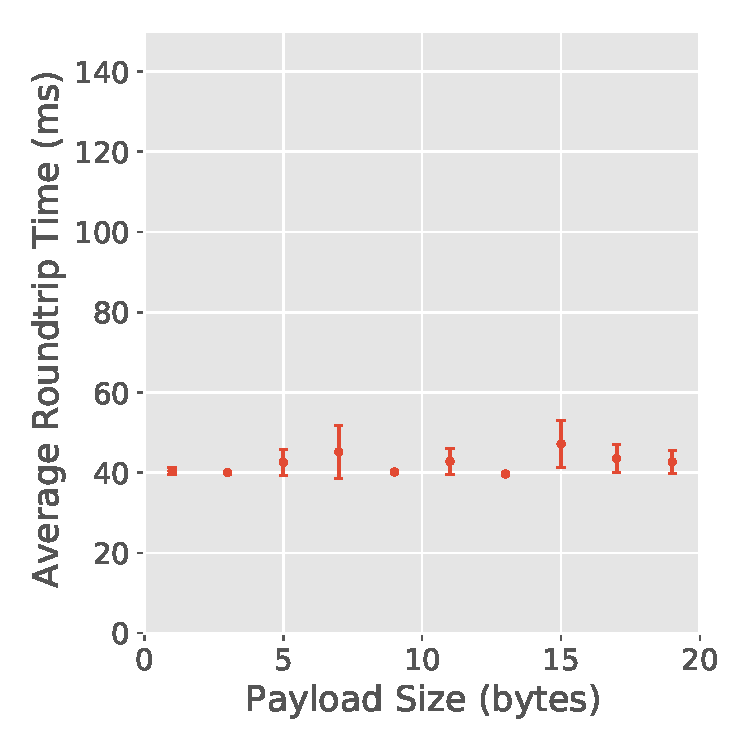
\includegraphics[width=\linewidth]{images/ble-roundtrip-hci1-300cm.pdf}
        \caption[Average \acs{BLE} connection roundtrip time obtained using the Raspberry Pi 4B's internal \acs{BLE} adapter at a distance of 3 m.]{Average \acs{BLE} connection roundtrip time obtained using Raspberry Pi 4B's internal \acs{BLE} adapter at a distance of $3\text{ m}$.}
        \label{fig:ble-roundtrip-hci1-3m}
    \end{minipage}
\end{figure}

\begin{figure}[H]
    \centering
    \begin{minipage}{0.45\linewidth}
        \centering
        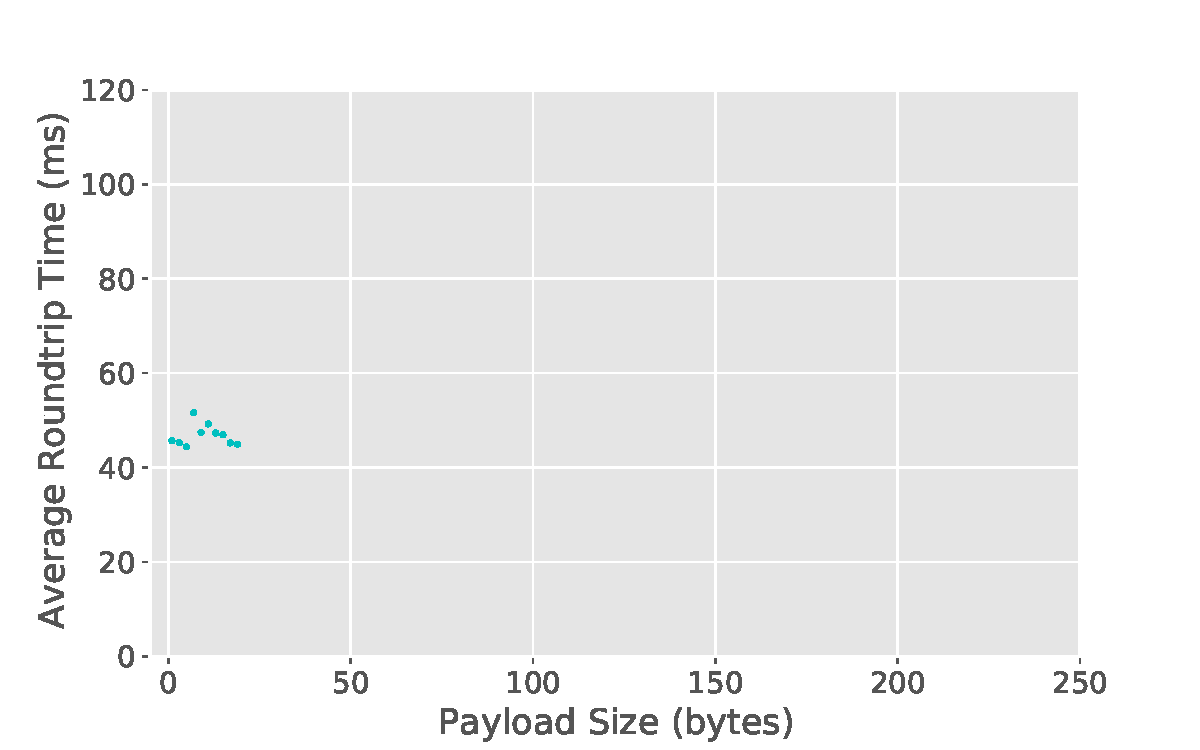
\includegraphics[width=\linewidth]{images/ble-roundtrip-hci1-600cm.pdf}
        \caption[Average \acs{BLE} connection roundtrip time obtained using the Raspberry Pi 4B's internal \acs{BLE} adapter at a distance of 6 m.]{Average \acs{BLE} connection roundtrip time obtained using Raspberry Pi 4B's internal \acs{BLE} adapter at a distance of $6\text{ m}$.}
        \label{fig:ble-roundtrip-hci1-6m}
    \end{minipage}
    \hspace{0.05\linewidth}
    \begin{minipage}{0.45\linewidth}
        \centering
        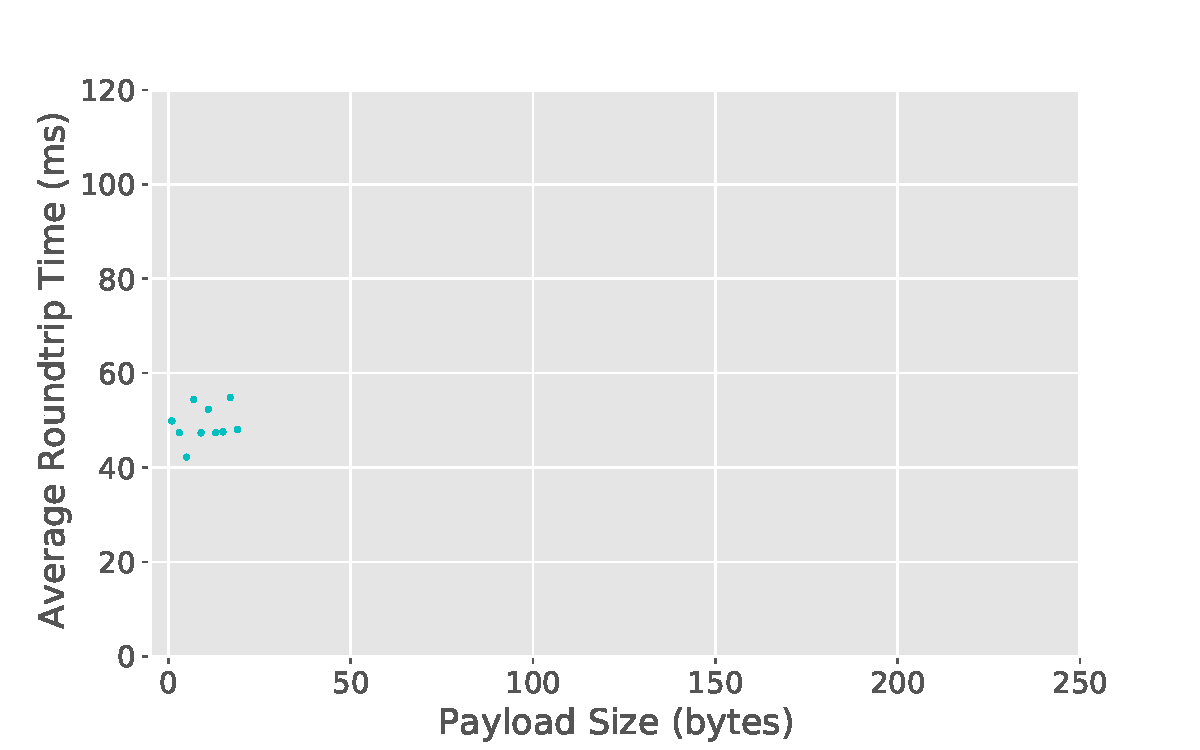
\includegraphics[width=\linewidth]{images/ble-roundtrip-hci1-900cm.pdf}
        \caption[Average \acs{BLE} connection roundtrip time obtained using the Raspberry Pi 4B's internal \acs{BLE} adapter at a distance of 9 m.]{Average \acs{BLE} connection roundtrip time obtained using Raspberry Pi 4B's internal \acs{BLE} adapter at a distance of $9\text{ m}$.}
        \label{fig:ble-roundtrip-hci1-9m}
    \end{minipage}
\end{figure}

\begin{figure}[H]
    \centering
    \begin{minipage}{0.45\linewidth}
        \centering
        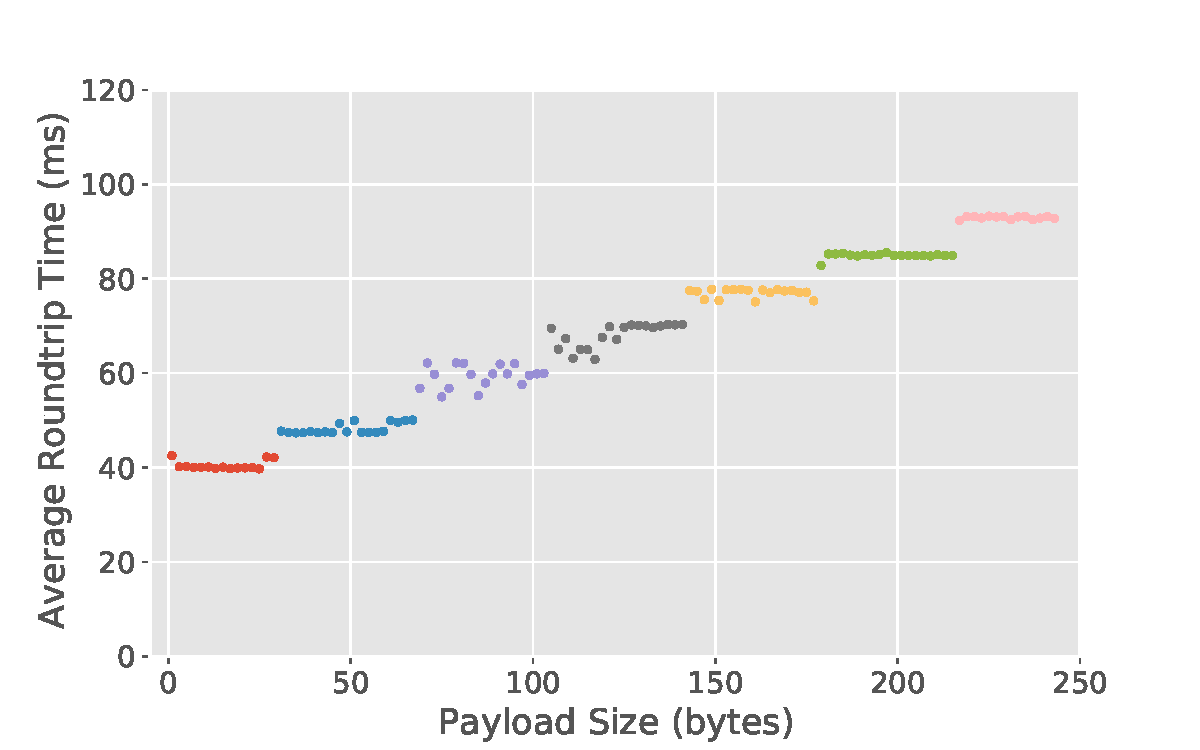
\includegraphics[width=\linewidth]{images/ble-roundtrip-hci0-0cm.pdf}
        \caption[Average \acs{BLE} connection roundtrip time obtained using the ASUS USB-BT500 adapter at a distance of 0 m.]{Average \acs{BLE} connection roundtrip time obtained using the ASUS USB-BT500 adapter at a distance of $0\text{ m}$. The data takes the shape similar to that of a ``stepping function'', as such, different colors are used to highlight clusters of data that correspond to different steps.}
        \label{fig:ble-roundtrip-hci0-0m}
    \end{minipage}
    \hspace{0.05\linewidth}
    \begin{minipage}{0.45\linewidth}
        \centering
        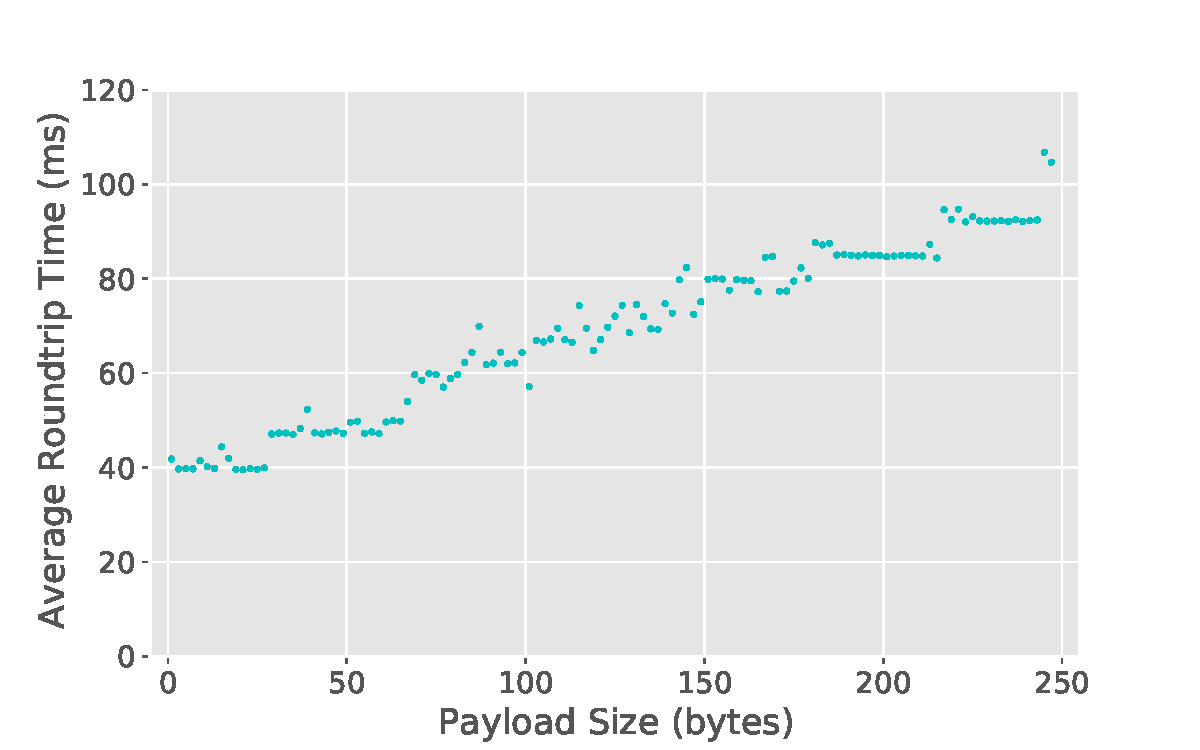
\includegraphics[width=\linewidth]{images/ble-roundtrip-hci0-300cm.pdf}
        \caption[Average \acs{BLE} connection roundtrip time obtained using the ASUS USB-BT500 adapter at a distance of 3 m.]{Average \acs{BLE} connection roundtrip time obtained using the ASUS USB-BT500 adapter at a distance of $3\text{ m}$. The data is colored according to the clusters of data found in Figure \ref{fig:ble-roundtrip-hci0-0m}.}
        \label{fig:ble-roundtrip-hci0-3m}
    \end{minipage}
\end{figure}

\begin{figure}[H]
    \centering
    \begin{minipage}{0.45\linewidth}
        \centering
        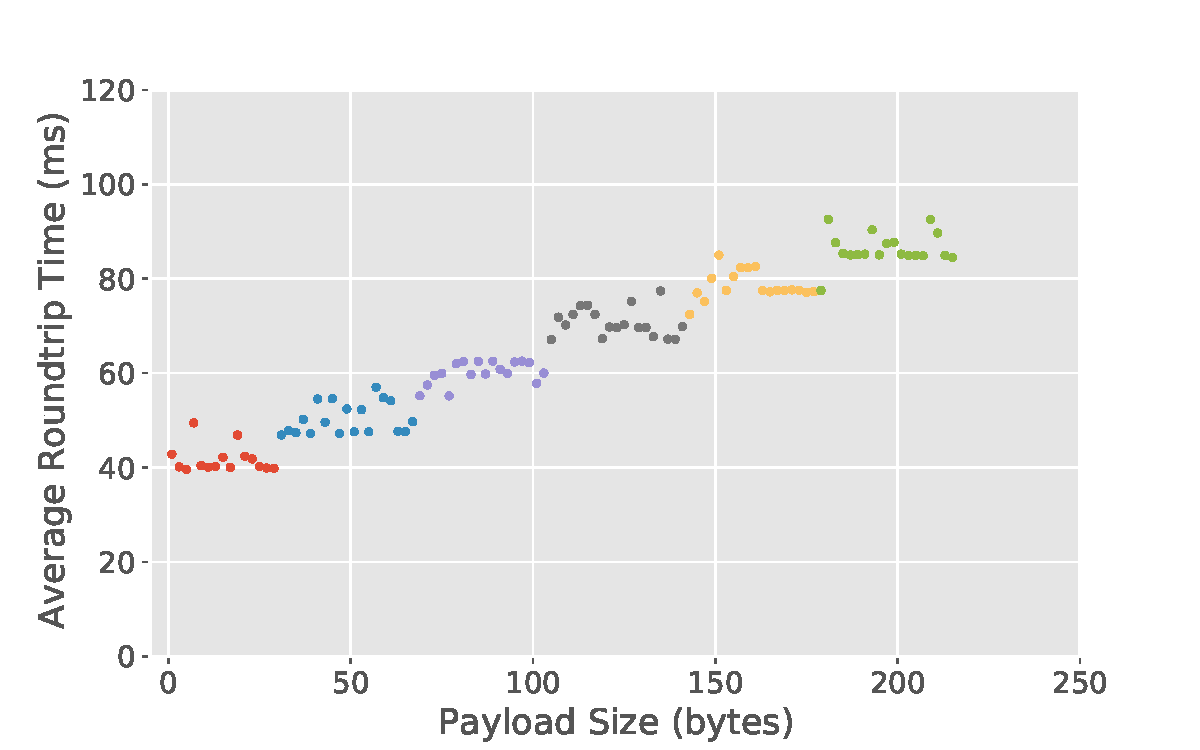
\includegraphics[width=\linewidth]{images/ble-roundtrip-hci0-600cm.pdf}
        \caption[Average \acs{BLE} connection roundtrip time obtained using the ASUS USB-BT500 adapter at a distance of 6 m.]{Average \acs{BLE} connection roundtrip time obtained using the ASUS USB-BT500 adapter at a distance of $6\text{ m}$. The data is colored according to the clusters of data found in Figure \ref{fig:ble-roundtrip-hci0-0m}.}
        \label{fig:ble-roundtrip-hci0-6m}
    \end{minipage}
    \hspace{0.05\linewidth}
    \begin{minipage}{0.45\linewidth}
        \centering
        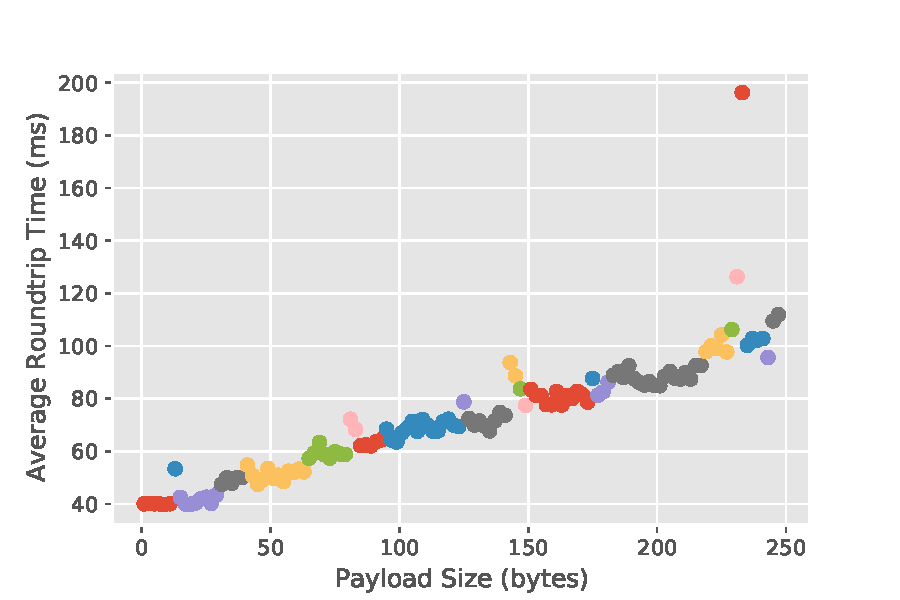
\includegraphics[width=\linewidth]{images/ble-roundtrip-hci0-900cm.pdf}
        \caption[Average \acs{BLE} connection roundtrip time obtained using the ASUS USB-BT500 adapter at a distance of 9 m.]{Average \acs{BLE} connection roundtrip time obtained using the ASUS USB-BT500 adapter at a distance of $9\text{ m}$. The data is colored according to the clusters of data found in Figure \ref{fig:ble-roundtrip-hci0-0m}.}
        \label{fig:ble-roundtrip-hci0-9m}
    \end{minipage}
\end{figure}

\paragraph{} Theoretically, the roundtrip time for different payload sizes in a \acs{BLE} connection should be a single line, or at most a step function as seen in Figure \ref{fig:ble-roundtrip-hci0-9m}. This occurs because the amount of radio time allocated for each connection event is limited according to the connection parameters that are exchanged by both devices. If the device is not capable of sending the entire message in the radio time allocated for a single \acs{PDU}, then it is fragmented over multiple \acs{PDU}s which can span over multiple Connection Events. Since these occur periodically according to the Connection Interval exchanged at the start of the connection, it creates the ``step'' effect mentioned. Additionally, even though the transmission time to exchange the payload increases linearly with the size of the payload, from the Application Layer standpoint, this may not be directly observed since most \acs{BLE} stacks handle the communication differently. All \acs{BLE} stacks used in these tests notify the Application Layer only after processing all radio events, therefore it should not be possible to receive a message and reply to it in the same Connection Event, thus the transmission of any message must take at least one Connection Interval to be received and processed by the device.

\paragraph{} In all tests, both adapters were observed to have a minimum roundtrip time: approximately 40 ms. This is a somewhat unexpected value, given that the connection interval is set to 7.5 ms. This means that the time it takes to transmit a single message and receive it on the \textit{Smart box} takes more than 4 connection intervals, which is more than double of what is expected: one interval for the transmission of the packet to the nRF52-DK and one interval to retrieve the packet, totaling $7.5+7.5=15$ ms + processing time overhead at the application level. Since the roundtrip time accounts for both the transmission and reception of the data packet, this indicates that a ${\sim} $12 ms delay exists in every transmission and reception of data.

\paragraph{} As discussed in Section \ref{sec:ble_test_conditions}, the \acs{DLE} functionality support gives a head start for the ASUS USB-BT500, as it is capable of sending over 10 times more data in a single packet, compared to the Raspberry Pi 4B's internal \acs{BLE} adapter, which does not support it. The roundtrip times measurements become significantly noisy as the distance increases, as expected, but it is particularly egregious as the payload size approaches the \acs{MTU} length on the ASUS USB-BT500 tests at 9 m in Figure \ref{fig:ble-roundtrip-hci0-9m}.

\paragraph{} As mentioned previously, the graphs for the ASUS USB-BT500 tests, in particular in Figure \ref{fig:ble-roundtrip-hci0-0m}, have a shape similar to that of a step function. By analyzing the data from Figure \ref{fig:ble-roundtrip-hci0-0m}, it is observed that each step has an average width of $36.2 \pm 0.98$ bytes, and a difference of $9.18 \pm 1.18$ ms (which is quite close to the connection interval, 7.5 ms). This likely indicates that the data is being fragmented on the \acs{L2CAP} layer every ${\sim} $36 bytes (\textit{i.e.} it is the maximum payload size that is being sent in a single connection event), and split across multiple connection intervals, instead of being transmitted in a single packet. Additionally, the fact that it increments in steps of 1 Connection Interval could also suggest that the fragmentation only occurs from one of the transmissions -- either the transmission from the adapter to the nRF52-DK or from nRF52-DK to the adapter. 

\paragraph{} Moreover, this could imply that the observed delay is most likely a bottleneck on the \textit{BlueZ} Linux \textit{API}, delaying the transmission of data from the user level to the lower levels of the \acs{BLE} protocol stack and vice versa, as the roundtrip time increases in increments of the connection interval (albeit slightly higher than it) with the payload size, which is the expected behavior, pointing to an issue on the \acs{BLE} stack implementation.

\paragraph{} Overall, it is observed that in order to maximize data throughput, the maximum supported payload size should be used in order to minimize the impact of the ${\sim} $12 ms delay on the transmission.

\subsubsection{Test 2: Bandwidth Measurement}

In this second test, the bandwidth for the \acs{BLE} connection is measured by adjusting the transmission rate of the data sent through the BLE channel, or more accurately, the time between the transmission of each packet. The test has been performed by reducing the time between transmissions from 500 ms to 10 ms, in 5 ms decrements, until the communication is stopped. In the graphs, this is converted to transmission rate in order to facilitate the interpretation of data.

\paragraph{} For this test, the nRF52-DK board exposes 7 \acs{GATT} characteristics for the \textit{Smart box} to subscribe to, which corresponds to the maximum amount of concurrent subscriptions using \textit{BlueZ}. This was determined empirically during the setup for the tests. The nRF52-DK then continuously changes the value of the characteristic, immediately triggering a notification to the \textit{Smart box} -- one for each characteristic. The transmission rate is increased until the limit of the connection, which eventually becomes too unstable and suddenly terminates. The payload size used on each characteristic corresponds to the maximum \acs{ATT} payload observed in the roundtrip test -- 20 bytes for the internal \acs{BLE} adapter and 244 bytes for the ASUS USB-BT500 adapter.

\paragraph{} Figures \crefrange{fig:ble-bandwidth-hci1-0m}{fig:ble-bandwidth-hci0-9m} show the bandwidth graphs obtained for each test configuration for each adapter. Each test configuration (\textit{i.e.} transmission rate and distance) has been run 3 times to ensure the consistency of results, for a total of $2376$ independent tests. 


\begin{figure}[H]
    \centering
    \begin{minipage}{0.45\linewidth}
        \centering
        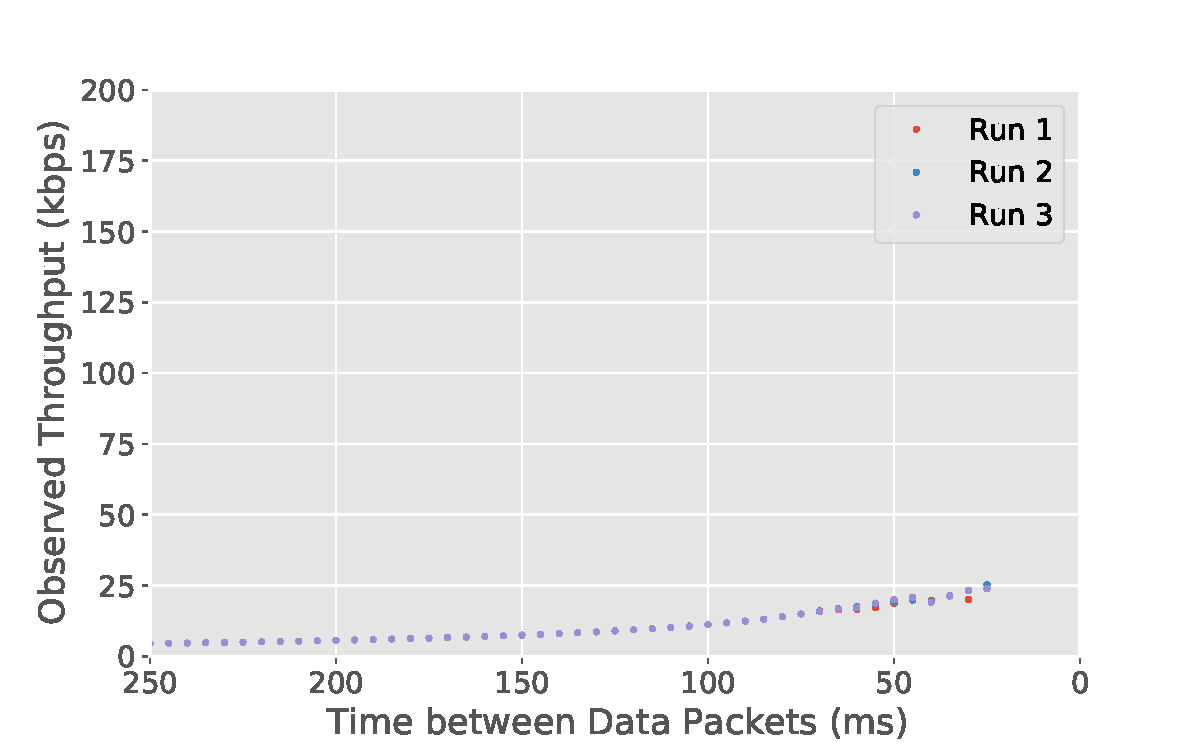
\includegraphics[width=\linewidth]{images/ble-bandwidth-hci1-0cm.pdf}
        \caption[\acs{BLE} connection bandwidth obtained using the ASUS USB-BT500 adapter at a distance of 0 m.]
        {\acs{BLE} connection bandwidth obtained using the Raspberry Pi 4B internal \acs{BLE} adapter at a distance of $0\text{ m}$. The maximum bandwidth achieved at this distance was $22.9 \pm 7.34$ kbps, achieved at 40 Hz with 43.5\% packet loss.}
        \label{fig:ble-bandwidth-hci1-0m}
    \end{minipage}
    \hspace{0.05\linewidth}
    \begin{minipage}{0.45\linewidth}
        \centering
        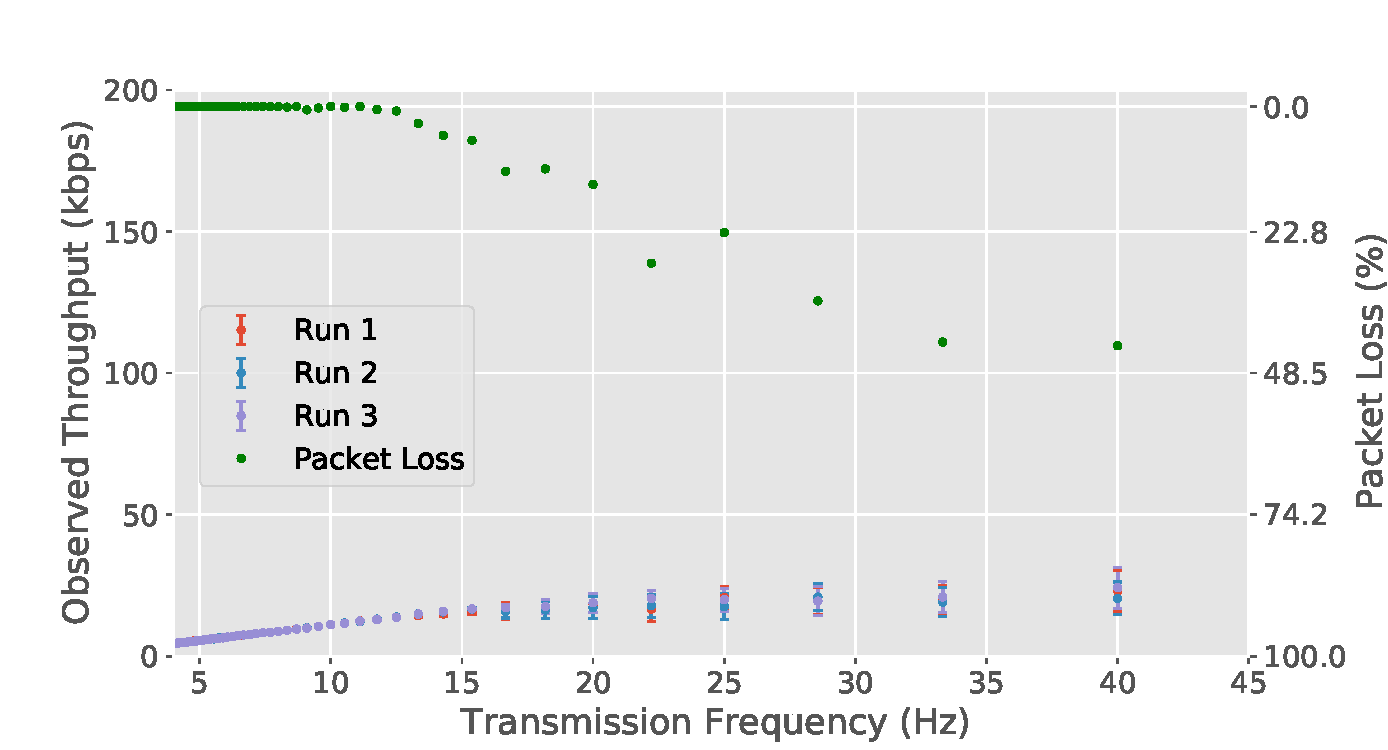
\includegraphics[width=\linewidth]{images/ble-bandwidth-hci1-300cm.pdf}
        \caption[\acs{BLE} connection bandwidth obtained using the ASUS USB-BT500 adapter at a distance of 3 m.]    {\acs{BLE} connection bandwidth obtained using the Raspberry Pi 4B internal \acs{BLE} adapter at a distance of 3 m. The maximum bandwidth achieved at this distance was $24.2 \pm 7.25$ kbps, achieved at 40 Hz with 41.0\% packet loss.}
        \label{fig:ble-bandwidth-hci1-3m}
    \end{minipage}
\end{figure}

\begin{figure}[H]
    \centering
    \begin{minipage}{0.45\linewidth}
        \centering
        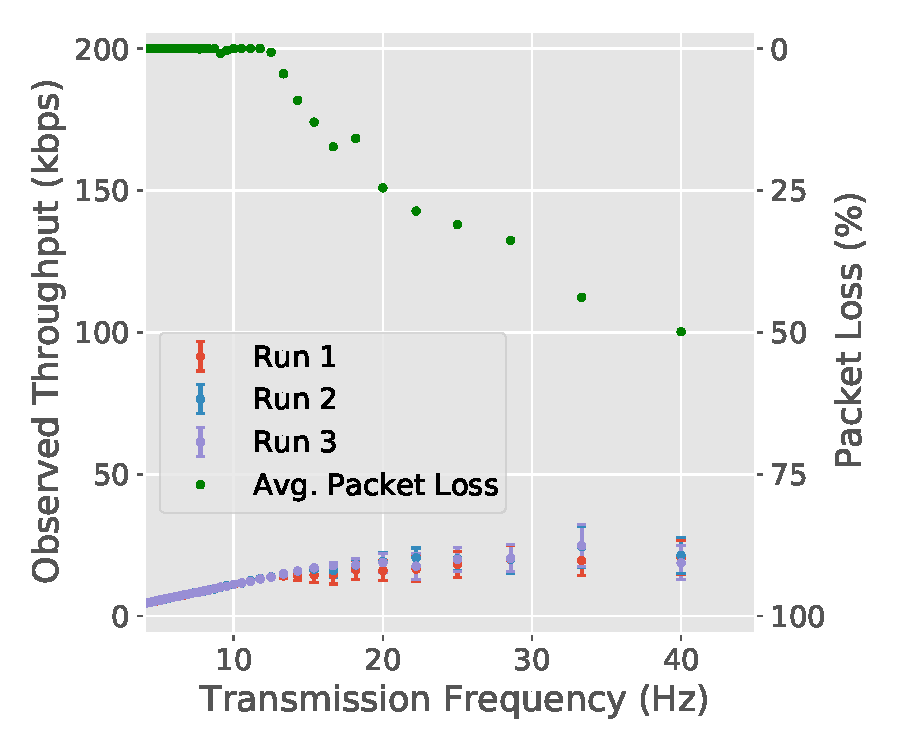
\includegraphics[width=\linewidth]{images/ble-bandwidth-hci1-600cm.pdf}
        \caption[\acs{BLE} connection bandwidth obtained using the ASUS USB-BT500 adapter at a distance of 6 m.]{\acs{BLE} connection bandwidth obtained using the Raspberry Pi 4B internal \acs{BLE} adapter at a distance of $6\text{ m}$. The maximum bandwidth achieved at this distance was $24.8 \pm 7.43$ kbps, achieved at 33.33 Hz with 27.2\% packet loss.}
        \label{fig:ble-bandwidth-hci1-6m}
    \end{minipage}
    \hspace{0.05\linewidth}
    \begin{minipage}{0.45\linewidth}
        \centering
        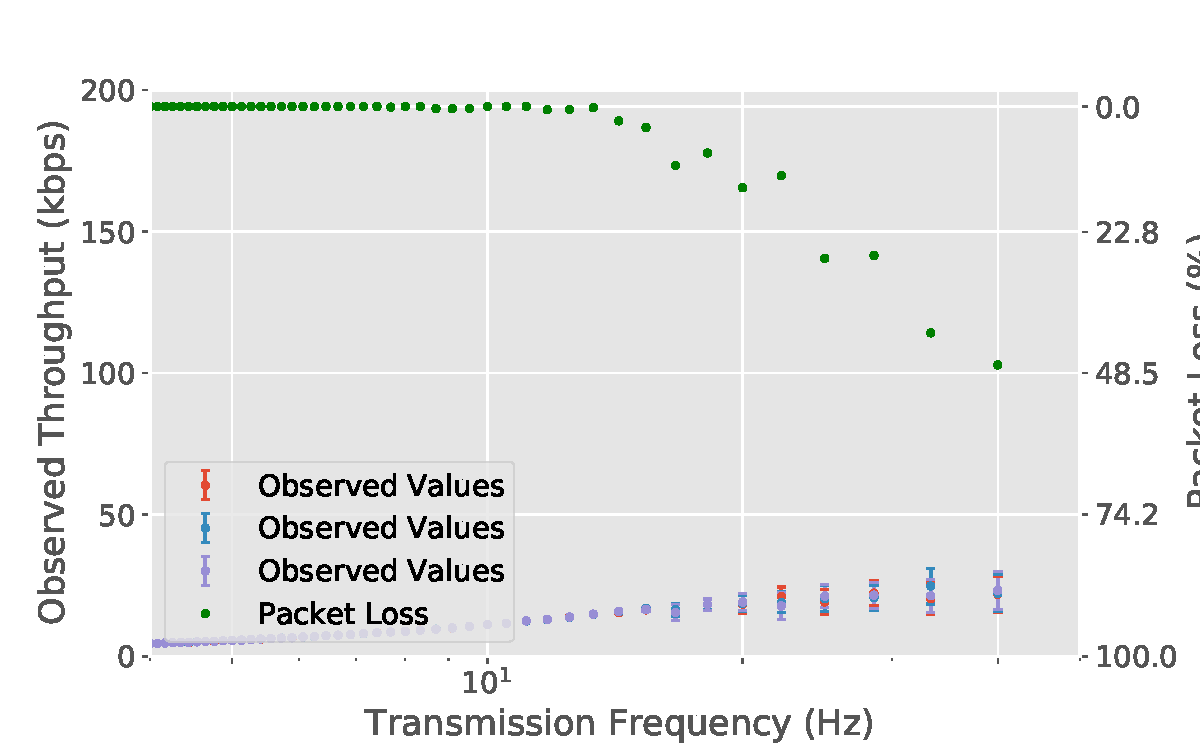
\includegraphics[width=\linewidth]{images/ble-bandwidth-hci1-900cm.pdf}
        \caption[\acs{BLE} connection bandwidth obtained using the ASUS USB-BT500 adapter at a distance of 9 m.]{\acs{BLE} connection bandwidth obtained using the Raspberry Pi 4B internal \acs{BLE} adapter at a distance of $9\text{ m}$. The maximum bandwidth achieved at this distance was $24.8 \pm 6.35$ kbps, achieved at 33.33 Hz with 28.9\% packet loss.}
        \label{fig:ble-bandwidth-hci1-9m}
    \end{minipage}
\end{figure}

\begin{figure}[H]
    \centering
    \begin{minipage}{0.45\linewidth}
        \centering
        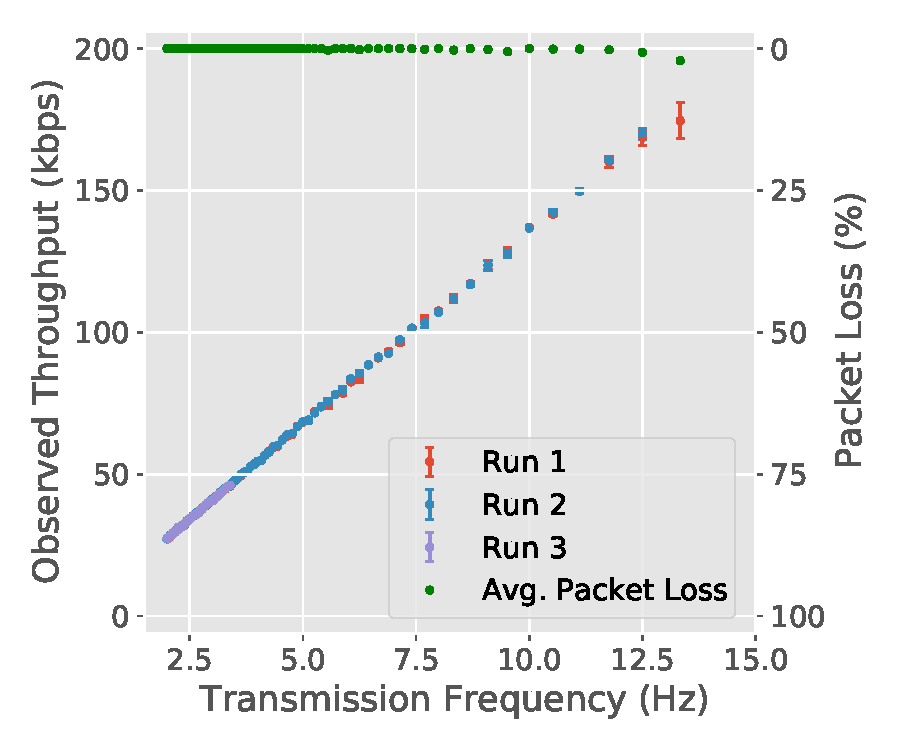
\includegraphics[width=\linewidth]{images/ble-bandwidth-hci0-0cm.pdf}
        \caption[\acs{BLE} connection bandwidth obtained using the ASUS USB-BT500 adapter at a distance of 0 m.]{\acs{BLE} connection bandwidth obtained using the ASUS USB-BT500 adapter at a distance of $0\text{ m}$. The maximum bandwidth achieved at this distance was $175.0 \pm 6.23$ kbps, achieved at 13.33 Hz with 2.13\% packet loss.}
        \label{fig:ble-bandwidth-hci0-0m}
    \end{minipage}
    \hspace{0.05\linewidth}
    \begin{minipage}{0.45\linewidth}
        \centering
        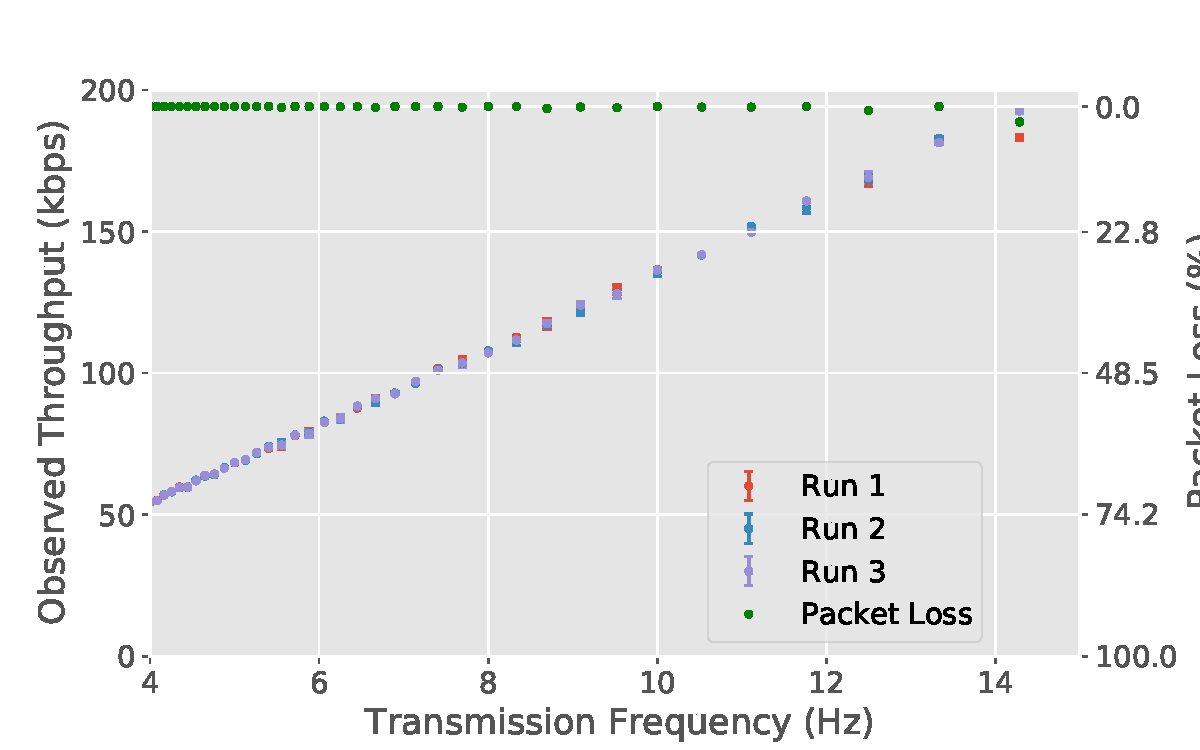
\includegraphics[width=\linewidth]{images/ble-bandwidth-hci0-300cm.pdf}
        \caption[\acs{BLE} connection bandwidth obtained using the ASUS USB-BT500 adapter at a distance of 3 m.]{\acs{BLE} connection bandwidth obtained using the ASUS USB-BT500 adapter at a distance of $3\text{ m}$. The maximum bandwidth achieved at this distance was $193.0 \pm 0.779$ kbps, achieved at 14.29 Hz with 0.25\% packet loss.}
        \label{fig:ble-bandwidth-hci0-3m}
    \end{minipage}
\end{figure}

\begin{figure}[H]
    \centering
    \begin{minipage}{0.45\linewidth}
        \centering
        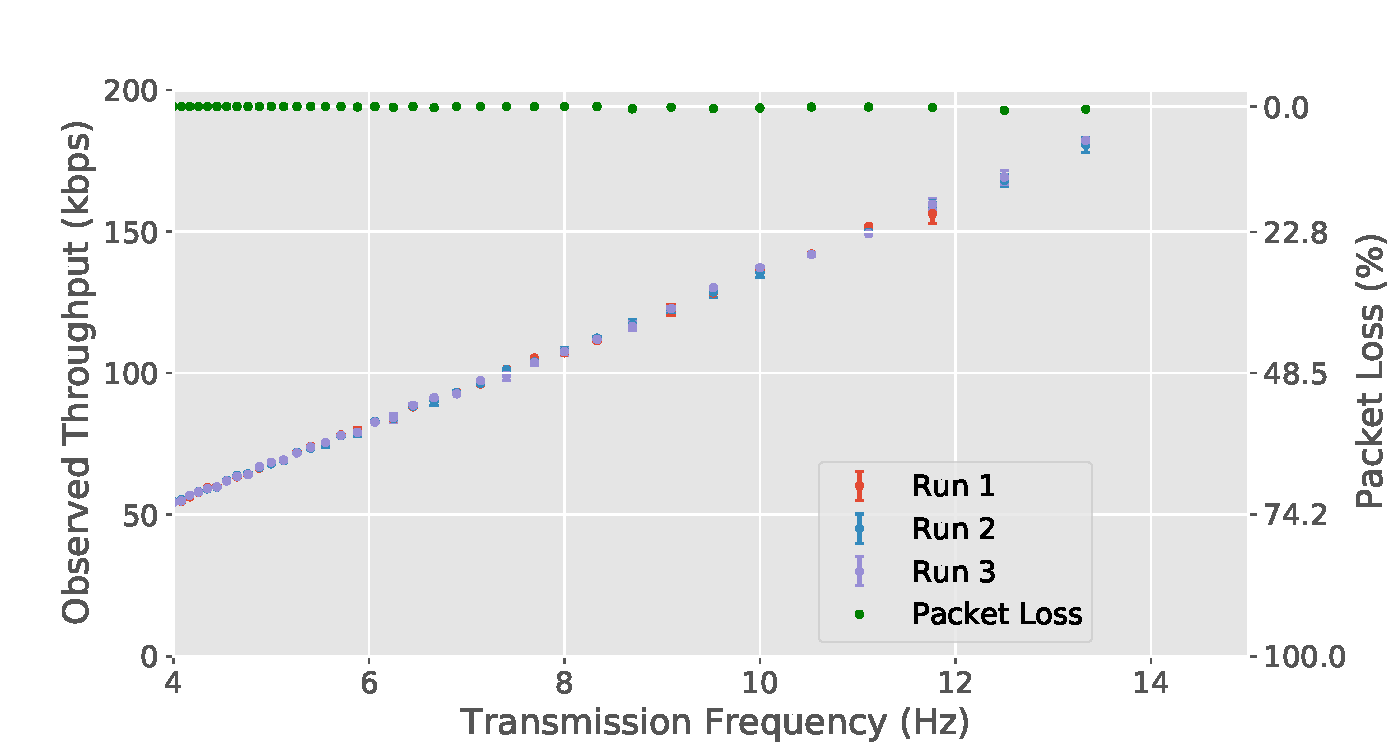
\includegraphics[width=\linewidth]{images/ble-bandwidth-hci0-600cm.pdf}
        \caption[\acs{BLE} connection bandwidth obtained using the ASUS USB-BT500 adapter at a distance of 6 m.]{\acs{BLE} connection bandwidth obtained using the ASUS USB-BT500 adapter at a distance of $6\text{ m}$. The maximum bandwidth achieved at this distance was $182.0 \pm 0.0132$ kbps, achieved at 13.33 Hz with 0\% packet loss.}
        \label{fig:ble-bandwidth-hci0-6m}
    \end{minipage}
    \hspace{0.05\linewidth}
    \begin{minipage}{0.45\linewidth}
        \centering
        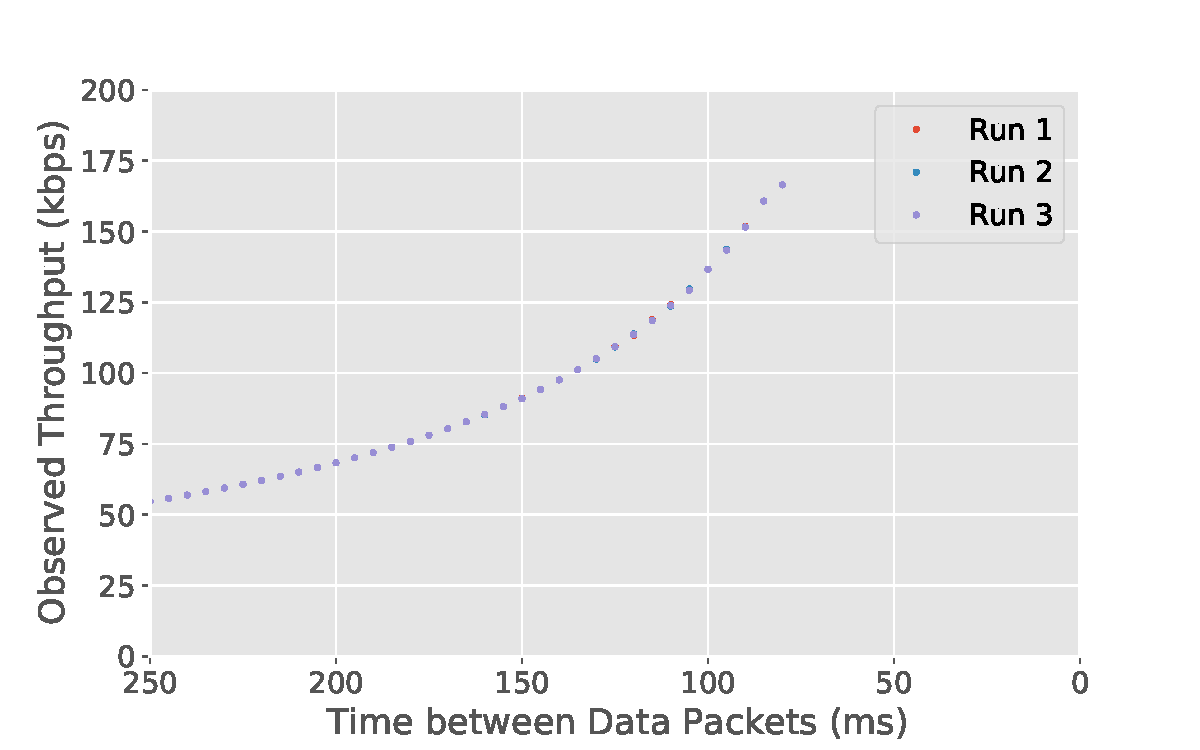
\includegraphics[width=\linewidth]{images/ble-bandwidth-hci0-900cm.pdf}
        \caption[\acs{BLE} connection bandwidth obtained using the ASUS USB-BT500 adapter at a distance of 9 m.]{\acs{BLE} connection bandwidth obtained using the ASUS USB-BT500 adapter at a distance of $9\text{ m}$. The maximum bandwidth achieved at this distance was $164.0 \pm 8.08$ kbps, achieved at 12.5 Hz with 2.53\% packet loss.}
        \label{fig:ble-bandwidth-hci0-9m}
    \end{minipage}
\end{figure}

\paragraph{} The maximum bandwidth for a \acs{BLE} connection can be estimated using the sequence diagram in Figure \ref{fig:ble-message-sequence-chart} and packet format in Figure \ref{fig:ble-ll-packet-format}. To simplify the calculation, it is assumed that the devices can transmit as much data as possible within the Connection Event, which is considered to be as long as the Connection Interval (7.5 ms). As mentioned in Section \ref{sec:ble_test_conditions}, all \acs{BLE} connections for these tests use LE 1M modulation, which has a bit rate of 1 Mbps. Additionally, the distance between the devices is also not considered in the calculation, as the time delay associated with distance is approximately 4 ns/m \cite{Specification1999} while the modulation time is 1 $\mu$s/bit, and therefore can be safely disregarded. Thus, the time to transmit a single \acs{BLE} message is:

\begin{equation}
    t_{TX} = (17 + p_{l}) \times 8\ \text{bits/byte} \times 1\ \mu\text{s}/\text{bit} = 8\times p_l + 136\ \mu\text{s,}
\end{equation}

where $p_{l}$ is the \acs{ATT} payload length. Since this packet must be acknowledged, two other factors must also be considered: 

\begin{enumerate}
    \item Time to transmit the acknowledgement packet, which has an empty \acs{ATT} payload and does not include the \acs{ATT} header: $t_{RX} = (1+4+3+2+4+1)\times 8 = 120\ \mu\text{s}$.
    \item Minimum time interval between consecutive packets on the same radio channel: $t_{IFS} = 150\ \mu\text{s}$.
\end{enumerate}

\paragraph{} Thus, the total time is:
\begin{equation}
    t_{t} = t_{TX}+ t_{IFS}+ t_{RX} + t_{IFS} =  8\times p_l  + 556\ \mu\text{s,}
\end{equation}

\paragraph{} With this information, a function to estimate the maximum throughput can be determined, by calculating the number of packets that can be transmitted in a single connection interval of 7.5 ms:

\begin{equation}
    B_{max} = \bigg\lfloor \frac{7.5\times 1000}{8\times p_l  + 556} \bigg\rfloor\times \frac{8\times p_l}{7.5}\ \text{kbps.}
\end{equation}

\paragraph{} This yields $B_{max}=213.33\ \text{kbps}$ for the payload length used in the internal adapter tests and $B_{max}=520.53\ \text{kbps}$ for the payload length used in the ASUS USB-BT500 tests, which are very different from those observed in the tests. Unfortunately, there are many factors which influence throughput, such as memory constraints on the \acs{BLE} implementations that limit the amount of messages that can be sent in single Connection Event, and other processing delays that impact the throughput \cite{Gomez2012}, which are extremely difficult to account for as the underlying causes are not evident most of the time. For example, in the roundtrip test a 12 ms delay is observed for transmission / reception of data, but it is not possible to determine exactly in which layer the delay (or delays) are occurring as the tools available for troubleshooting these issues on Linux are limited.

\paragraph{} Additionally, packet loss can be observed as transmission frequency increases, reaching closer to the ``breaking point'' where the connection suddenly crashes, as expected. However, the internal \acs{BLE} adapter shows a much more noticeable packet loss (particularly when the transmission frequency is greater than 15 Hz). This, coupled with the analysis of the previous tests, likely indicates that these losses are caused by limitations of the \acs{BLE} stack rather than the adapter itself, \textit{i.e.} the existing \acs*{BLE} implementation cannot handle these high transmission rates properly, and higher payload sizes are preferred instead. This would also explain why the packet loss is nearly 0\% for the ASUS USB-BT500 tests before reaching the ``breaking point'', since it uses a much higher payload size.

\paragraph{} Using these tests, it is possible to determine the adequacy of these adapters for handling the \acs*{BLE} communication with the \textit{Biostickers} using the data sizes and transmission frequencies from Section \ref{sec:biosticker_data}, where it is seen that the communication with the \textit{Biostickers} uses close to 3.593 kbps of bandwidth. Both adapters are more than capable of handling that bandwidth, for any distance up to 9 meters, however, they cannot reach the 20 Hz transmission frequency required by the ECG data communication without significant packet loss due to limitations of the \acs{BLE} stack, as discussed previously. In order to use the \textit{Biostickers} without packet loss, the data must be grouped and sent in larger packets, thus lowering the transmission rate and increasing the packet size in order to bypass these limitations, however this approach is only possible using the ASUS USB-BT500 \acs{BLE} adapter. 

\paragraph{} Curiously, some graphs show better throughput for intermediate distances rather when the devices are next to each other, \text{e.g.} for Figure \ref{fig:ble-bandwidth-hci1-0m} at 0 m and \ref{fig:ble-bandwidth-hci1-3m} at 3 m. This is likely caused by misalignment of the devices, which can slightly improve the efficiency of the power transfer in radio transmissions (as no information about the \acs{BLE} adapter antennas is known), improving the stability of the connection and thus allowing the usage of a higher transmission rate before the connection crashes. Moreover, as expected from the previous tests, ASUS USB-BT500 shows a much better throughput since it can transmit more data in the \acs{LL} data packets. 

\subsection{Decision on the \acs{BLE} adapter}

From the previous tests, it is observed that the Raspberry Pi 4B's internal \acs{BLE} adapter lacks the support for \acs{DLE} feature, which reduces greatly the communication throughput. Additionally, this maximum throughput on Raspberry Pi 4B is achieved with an extremely high packet loss (over 40\%). This suggests that to make full use of this adapter, the system and communications must be designed considering this packet loss, or reduce the \acs{BLE} throughput to minimize the packet loss. The ASUS USB-BT500 on the other hand has a throughput 10 times larger than the internal adapter, with very low packet loss (which can be mitigated by slightly reducing the throughput).

\paragraph{} Due to all the aforementioned reasons, the ASUS USB-BT500 adapter was chosen for the development of \acs{BLE} data acquisition in the scope of the \acs{WoW} project.

\section{Summary}
In this chapter, a comprehensive performance study of the different \acs{SBC}s considered for the \textit{Smart box} development was presented, as well as an extensive analysis of the \acs{BLE} data communication.

\paragraph{} In the next chapter, the development of the next component in the proposed \acs{IoT} architecture is presented -- the \textit{Smart Gateway}.